%%%%%%%%%%%%%%%%%%%%%%%%%%%%%%%%%%%%%%%%%12pt: grandezza carattere
                                        %a4paper: formato a4
                                        %openright: apre i capitoli a destra
                                        %twoside: serve per fare un
                                        %   documento fronteretro
                                        %report: stile tesi (oppure book)
\documentclass[12pt,a4paper,openright,twoside]{report}
%
%%%%%%%%%%%%%%%%%%%%%%%%%%%%%%%%%%%%%%%%%libreria per scrivere in italiano
\usepackage[italian]{babel}
%
%%%%%%%%%%%%%%%%%%%%%%%%%%%%%%%%%%%%%%%%%libreria per accettare i caratteri
                                        %   digitati da tastiera come � �
                                        %   si pu� usare anche
                                        %   \usepackage[T1]{fontenc}
                                        %   per� con questa libreria
                                        %   il tempo di compilazione
                                        %   aumenta
\usepackage[utf8x]{inputenc}
%
%%%%%%%%%%%%%%%%%%%%%%%%%%%%%%%%%%%%%%%%%libreria per impostare il documento
\usepackage{fancyhdr}
%
%%%%%%%%%%%%%%%%%%%%%%%%%%%%%%%%%%%%%%%%%libreria per avere l'indentazione
%%%%%%%%%%%%%%%%%%%%%%%%%%%%%%%%%%%%%%%%%   all'inizio dei capitoli, ...
\usepackage{indentfirst}
%
%%%%%%%%%libreria per mostrare le etichette
%\usepackage{showkeys}
%
%%%%%%%%%%%%%%%%%%%%%%%%%%%%%%%%%%%%%%%%%libreria per inserire grafici
\usepackage{graphicx}
%
%%%%%%%%%%%%%%%%%%%%%%%%%%%%%%%%%%%%%%%%%libreria per utilizzare font
                                        %   particolari ad esempio
                                        %   \textsc{}
\usepackage{newlfont}
%
%%%%%%%%%%%%%%%%%%%%%%%%%%%%%%%%%%%%%%%%%librerie matematiche
\usepackage{amssymb}
\usepackage{amsmath}
\usepackage{latexsym}
\usepackage{amsthm}

\usepackage{tabularx}

\usepackage[dvipsnames]{xcolor}

\usepackage{listings}
\usepackage{color}
\usepackage{dblfloatfix}

\definecolor{dkgreen}{rgb}{0,0.6,0}
\definecolor{gray}{rgb}{0.5,0.5,0.5}
\definecolor{mauve}{rgb}{0.58,0,0.82}

\lstset{frame=tb,
  language=Java,
  aboveskip=3mm,
  belowskip=3mm,
  showstringspaces=false,
  columns=flexible,
  basicstyle={\small\ttfamily},
  numbers=none,
  numberstyle=\tiny\color{gray},
  keywordstyle=\color{blue},
  commentstyle=\color{dkgreen},
  stringstyle=\color{mauve},
  breaklines=true,
  breakatwhitespace=true,
  tabsize=3
}

\lstdefinelanguage{JavaScript}{
  keywords={typeof, new, true, false, catch, function, return, null, catch, switch, var, if, in, while, do, else, case, break},
  keywordstyle=\color{blue}\bfseries,
  ndkeywords={class, export, boolean, throw, implements, import, this},
  ndkeywordstyle=\color{darkgray}\bfseries,
  identifierstyle=\color{black},
  sensitive=false,
  comment=[l]{//},
  morecomment=[s]{/*}{*/},
  commentstyle=\color{purple}\ttfamily,
  stringstyle=\color{red}\ttfamily,
  morestring=[b]',
  morestring=[b]"
}

\lstdefinestyle{json}
{
  showstringspaces    = false,
  keywords            = {false,true},
  alsoletter          = 0123456789.,
  morestring          = [s]{"}{"},
  stringstyle         = \ifcolonfoundonthisline\JSONstringvaluestyle\fi,
  MoreSelectCharTable =%
    \lst@DefSaveDef{`:}\colon@json{\processColon@json},
  basicstyle          = \ttfamily,
  keywordstyle        = \ttfamily\bfseries,
}

\lstdefinelanguage{Kotlin}{
  keywords={package, as, typealias, this, super, val, var, fun, for, null, true, false, is, in, throw, return, break, continue, object, if, try, else, while, do, when, yield, typeof, yield, typeof, class, interface, enum, object, override, public, private, get, set, import, abstract, },
  keywordstyle=\color{NavyBlue}\bfseries,
  ndkeywords={@Deprecated, Iterable, Int, Integer, Float, Double, String, Runnable, dynamic},
  ndkeywordstyle=\color{BurntOrange}\bfseries,
  emph={println, return@, forEach,},
  emphstyle={\color{OrangeRed}},
  identifierstyle=\color{black},
  sensitive=true,
  commentstyle=\color{gray}\ttfamily,
  comment=[l]{//},
  morecomment=[s]{/*}{*/},
  stringstyle=\color{ForestGreen}\ttfamily,
  morestring=[b]",
  morestring=[s]{"""*}{*"""},
}



\oddsidemargin=30pt \evensidemargin=20pt%impostano i margini
\hyphenation{sil-la-ba-zio-ne pa-ren-te-si}%serve per la sillabazione: tra parentesi
					   %vanno inserite come nell'esempio le parole
%					   %che latex non riesce a tagliare nel modo giusto andando a capo.

%
%%%%%%%%%%%%%%%%%%%%%%%%%%%%%%%%%%%%%%%%%comandi per l'impostazione
                                        %   della pagina, vedi il manuale
                                        %   della libreria fancyhdr
                                        %   per ulteriori delucidazioni
\pagestyle{fancy}\addtolength{\headwidth}{20pt}
\renewcommand{\chaptermark}[1]{\markboth{\thechapter.\ #1}{}}
\renewcommand{\sectionmark}[1]{\markright{\thesection.\ #1}{}}
\rhead[\fancyplain{}{\bfseries\leftmark}]{\fancyplain{}{\bfseries\thepage}}
\cfoot{}
%%%%%%%%%%%%%%%%%%%%%%%%%%%%%%%%%%%%%%%%%
\linespread{1.3}                        %comando per impostare l'interlinea
%%%%%%%%%%%%%%%%%%%%%%%%%%%%%%%%%%%%%%%%%definisce nuovi comandi
%
\begin{document}


 \documentclass[12pt,a4paper]{report}
\usepackage[italian]{babel}
\usepackage{newlfont}
\textwidth=450pt\oddsidemargin=0pt
\begin{document}
\begin{titlepage}
\begin{center}
{{\Large{\textsc{Alma Mater Studiorum $\cdot$ Universit\`a di
Bologna}}}} \rule[0.1cm]{15.8cm}{0.1mm}
\rule[0.5cm]{15.8cm}{0.6mm}
{\small{\bf SCUOLA DI SCIENZE\\
Corso di Laurea in Nome corso di Laurea }}
\end{center}
\vspace{15mm}
\begin{center}
{\LARGE{\bf TITOLO}}\\
\vspace{3mm}
{\LARGE{\bf DELLA}}\\
\vspace{3mm}
{\LARGE{\bf TESI}}\\
\end{center}
\vspace{40mm}
\par
\noindent
\begin{minipage}[t]{0.47\textwidth}
{\large{\bf Relatore:\\
Chiar.mo Prof.\\
NOME RELATORE}}
\end{minipage}
\hfill
\begin{minipage}[t]{0.47\textwidth}\raggedleft
{\large{\bf Presentata da:\\
NOME LAUREANDO}}
\end{minipage}
\vspace{20mm}
\begin{center}
{\large{\bf Sessione\\%inserire il numero della sessione in cui ci si laurea
Anno Accademico }}%inserire l'anno accademico a cui si � iscritti
\end{center}
\end{titlepage}
\end{document}

 \begin{titlepage}                       %crea un ambiente libero da vincoli
                                        %   di margini e grandezza caratteri:
                                        %   si pu\`o modificare quello che si
                                        %   vuole, tanto fuori da questo
                                        %   ambiente tutto viene ristabilito
%
\thispagestyle{empty}                   %elimina il numero della pagina
\topmargin=6.5cm                        %imposta il margina superiore a 6.5cm
\raggedleft                             %incolonna la scrittura a destra
\large                                  %aumenta la grandezza del carattere
                                        %   a 14pt
\em                                     %emfatizza (corsivo) il carattere
A Claudio Maracci \ldots                      %\ldots lascia tre puntini
\newpage                                %va in una pagina nuova
%
%%%%%%%%%%%%%%%%%%%%%%%%%%%%%%%%%%%%%%%%
\clearpage{\pagestyle{empty}\cleardoublepage}%non numera l'ultima pagina sinistra
\end{titlepage}

 \pagenumbering{roman}                   %serve per mettere i numeri romani
\tableofcontents                        %crea l'indice
%%%%%%%%%%%%%%%%%%%%%%%%%%%%%%%%%%%%%%%%%imposta l'intestazione di pagina
\rhead[\fancyplain{}{\bfseries\leftmark}]{\fancyplain{}{\bfseries\thepage}}
\lhead[\fancyplain{}{\bfseries\thepage}]{\fancyplain{}{\bfseries
INDICE}}
%%%%%%%%%%%%%%%%%%%%%%%%%%%%%%%%%%%%%%%%%non numera l'ultima pagina sinistra
\clearpage{\pagestyle{empty}\cleardoublepage}
\listoffigures                          %crea l'elenco delle figure
%%%%%%%%%%%%%%%%%%%%%%%%%%%%%%%%%%%%%%%%%non numera l'ultima pagina sinistra
\clearpage{\pagestyle{empty}\cleardoublepage}
\listoftables                           %crea l'elenco delle tabelle
%%%%%%%%%%%%%%%%%%%%%%%%%%%%%%%%%%%%%%%%%non numera l'ultima pagina sinistra
\clearpage{\pagestyle{empty}\cleardoublepage}

 \chapter*{Introduzione}                 %crea l'introduzione (un capitolo
                                        %   non numerato)

%%%%%%%%%%%%%%%%%%%%%%%%%%%%%%%%%%%%%%%%%imposta l'intestazione di pagina
\rhead[\fancyplain{}{\bfseries
Introduzione}]{\fancyplain{}{\bfseries\thepage}}
\lhead[\fancyplain{}{\bfseries\thepage}]{\fancyplain{}{\bfseries
INTRODUZIONE}}
%%%%%%%%%%%%%%%%%%%%%%%%%%%%%%%%%%%%%%%%%aggiunge la voce Introduzione
                                        %   nell'indice
\addcontentsline{toc}{chapter}{Introduzione}
L'idea di realizzare un'applicazione gestionale su piattaforma Android, è nata dall'esigenza di risolvere alcune problematiche reali riscontrate durante l'organizzazione di eventi, spese e commissioni da svolgere fra gruppi di persone.\\
Lo sviluppo iniziale si avvaleva di Java come linguaggio di programmazione, successivamente con l'annuncio ufficiale a Maggio 2017 del supporto di Google a Kotlin, come nuovo linguaggio di programmazione per Android, l'applicazione è stata riscritta completamente, utilizzando Kotlin.\\
Lo sviluppo dell'applicazione in Kotlin ha permesso di  analizzare le funzionalità del nuovo linguaggio sia teoricamente che con un'implementazione pratica che ha rendendo possibile anche un confronto diretto con Java.\\
In questa tesi verranno illustrate le principali funzionalità e caratteristiche del linguaggio Kotlin, e del BaaS Firebase utilizzato per la gestione della parte server. Dal terzo capitolo invece verrà presa in considerazione l'applicazione realizzata per lo studio di Kotlin, mostrando un architettura ad alto livello dell'infrastruttura dei servizi server e delle funzionalità dell'applicazione. Successivamente verranno analizzate porzioni di codice rilevani e discusse le implementazioni sviluppate per la realizzazione dell'applicazione. Infine nell'ultimo capitolo viene descritto l'attuale stato dell'arte, il confronto fra Java e Kotlin ed eventuali sviluppi futuri.
%%%%%%%%%%%%%%%%%%%%%%%%%%%%%%%%%%%%%%%%%non numera l'ultima pagina sinistra
\clearpage{\pagestyle{empty}\cleardoublepage}

 \chapter{Kotlin}                %crea il capitolo
%%%%%%%%%%%%%%%%%%%%%%%%%%%%%%%%%%%%%%%%%imposta l'intestazione di pagina
\lhead[\fancyplain{}{\bfseries\thepage}]{\fancyplain{}{\bfseries\rightmark}}
\pagenumbering{arabic}                  %mette i numeri arabi
\section{Storia}                 %crea la sezione

Kotlin \'e un linguaggio di programmazione open-source \footnote{https://github.com/JetBrains/kotlin}, con la caratteristica di essere orientato agli oggetti, staticamente tipizzato  e basato sulla JVM ( Java Virtual Machine).\\
Lo sviluppo di Kotlin \'e iniziato nel 2010 dall'azienda JetBrains, conosciuta nel modo dello sviluppo software per la realizzazione di diversi IDE ( Integrated development environment ), tra cui: Intellij IDEA,, sul quale si basa l'attuale IDE ufficiale di Google dedicato alla programmazione Android, chiamato: Android Studio.Java \'e sempre stato, negli ultimi anni, uno dei linguaggii  pi\'u usati e conosciuti ma presenta diverse imperfezioni e problemi che spinse il team di JetBrains a iniziare lo sviluppo di un suo linguaggio di programmazione che prendesse in considerazione alcuni spunti e idee introdotte da linguaggi preesistenti come CSharp, Scala, Groovy, ECMAScript, Go, Python.\\
Nel 2015 Google prese in considerazione l'utilizzo di Kotlin come plugin per Android-Studio, e dopo vari test nel 2017  durante la conferenza Google IO ( 2017 ), arriv\'o l'annuncio che uficcializzava Kotlin come nuovo linguaggio di programmazione per lo sviluppo di applicazioni Android, senza escludere e rinunciare a Java, su cui si basa attualmente l'SDK di Android.


\section{Caratteristiche}
Il linguaggio Kotlin \'e stato sviluppato per risolvere molti problemi tipici che riscontrano spesso programmatori Java, infatto  \'e stato progettato e progressivamente testato per 7 anni come versione "beta" dagli stessi programmatori che lavoravano presso JetBrains, fino a raggiungere nel 2017 la versione stabile, \'e nato quindi all'interno di un team di sviluppatori che hanno cercato di risolvere i loro stessi problemi e non in ambito di ricerca come spesso accade.\\
Kotlin prendendo spunto dalle problematiche di Java e da buone regole introdotte da alcuni linguaggi imperativi e funzionali \'e stato modellato in modo tale da aggiungere funzionalit\'a utili sia a livello sintattico che a livello prestazionale, offrendo quindi al programmatore strumenti, caratteristiche e implementazioni semplici e utili ma molto potenti.\\
Un altro aspetto importante su cui il team di Kotlin ha prestato molta attenzione è stata la cura e la buona integrazione del suo plugin con Android Studio. Il supporto dato dal plugin \'e quello di aiutare in ogni momento lo sviluppatore, consigliando tecniche di buona programmazione, abbreviazione del codice per rendere il tutto pi\'u coinciso, conversione automatica del codice Java in Kotlin e ove possibile cercher\'a di allertare lo sviluppatore su possibili errori e problemi di prestazione e sintattici.
Le caratteristiche pi\'u importanti offerte da Kotlin sono l'interoperabilit\'a con Java, permettendo l'utilizzo di librerie Java e Kotlin simultaneamente, l'introduzione di alcune caratteristiche dei linguaggi di ordine superiore, la tipizzazione statica delle variabili, l'inferenza di tipo e soprattutto il null-safety permettendo di differenziare il tipo nullabile e il tipo non-nullabile, prevenendo quindi errori di null pointer expetions.\\
Il codice prodotto in Kotlin \`e inoltre pi\'u compatto, coninciso e meno verboso grazie alle dataclass, il supporto delle lambda function e altri costrutti.





%https://superkotlin.com/why-kotlin-is-the-best-language-for-android-development/
\subsection{Interoperabilit\'a}
I linguaggi Kotlin e Java sono fortemente intercompatibili permettendo quindi a entrambi i linguaggi di coesistere all'interno dello stesso codice e di richimare funzioni e parti di codice in Java da Kotlin e viceversa, poich\'e entrambi i linguaggi producono Java Bytecode.\\
%http://kotlinlang.org/docs/reference/java-interop.html
Prendiamo in considerazione il classico esempio "Hello word" scritto in Kotlin e in Java

\begin{lstlisting}[language=java,caption={Hello.kt in Kotlin}]
package demo
fun main(args : Array<String>) {
  println("Hello, world!")
}
\end{lstlisting}

\begin{lstlisting}[language=java,caption={Hello.java in Java}]

public class HelloWorld {
    public static void main(String[] args) {
        System.out.println("Hello, world!");
    }
}
\end{lstlisting}

Il compilatore di Kotlin prendendo come input il file "Hello.kt" produrr\'a un JAR eseguibile da Java "Hello.jar"


\begin{lstlisting}[language=bash,caption={Compilatore kotlin}]
$ kotlinc Hello.kt -include-runtime -d Hello.jar //
$ java -jar Hello.jar
$ Hello, world!
\end{lstlisting}

 -includeruntime \'e un opzione del compilatore per produrre un eseguibile jar, includendo le runtime di Kotlin (~800Kb)
% Il compilatore di Kotlin permette inoltre di generare il java bytecode
% \begin{lstlisting}[language=bash,caption={Compilatore kotlin per generare Hello.class}]
% $ kotlinc HelloWorld.kt
% $ javap -c Hello.class
% \end{lstlisting}
%
% Confrontando
% \begin{lstlisting}[language=java,caption={Java Bitecode generato da Kotlin}]
%
% public final class demo.HelloKt {
%   public static final void main(java.lang.String[]);
%     Code:
%        0: aload_0
%        1: ldc           #9                  // String args
%        3: invokestatic  #15                 // Method kotlin/jvm/internal/Intrinsics.checkParameterIsNotNull:(Ljava/lang/Object;Ljava/lang/String;)V
%        6: ldc           #17                 // String Hello, world!
%        8: astore_1
%        9: getstatic     #23                 // Field java/lang/System.out:Ljava/io/PrintStream;
%       12: aload_1
%       13: invokevirtual #29                 // Method java/io/PrintStream.println:(Ljava/lang/Object;)V
%       16: return
% }
%
% \end{lstlisting}


% \begin{lstlisting}[language=java,caption={Java Bitecode generato da Kotlin}]
%
% class Hello {
%   Hello();
%     Code:
%        0: aload_0
%        1: invokespecial #1                  // Method java/lang/Object."<init>":()V
%        4: return
%
%   public static void main(java.lang.String[]);
%     Code:
%        0: getstatic     #2                  // Field java/lang/System.out:Ljava/io/PrintStream;
%        3: ldc           #3                  // String Hello, world!
%        5: invokevirtual #4                  // Method java/io/PrintStream.println:(Ljava/lang/String;)V
%        8: return
% }
%
%
% \end{lstlisting}





\subsection{Variabili}
Java pone due differenze quando si parla di variabili, mette a disposizione i principali tipi primitivi (int, boolean, byte, long, short, float, double, char) e i le loro corrispondenti classi (Int, Boolean, Byte, Long, Short, Float, Double, Char).
Uno dei principali cambiamenti introdotti da Kotlin \'e stato quello di rendere accessibile allo sviluppatore tutte le varibili come se fossero oggetti.\\
%https://docs.oracle.com/javase/1.5.0/docs/guide/language/autoboxing.html
La differenza fra i tipi primitivi e gli oggetti sta nel fatto che i primi indicano solamente il tipo di una variabile, mentre gli oggetti incapsulano il tipo e ne aggiungono funzionalit\'a e metodi aggiuntivi, inoltre il tipo primitivo non pu\'o assumere valore nullo. \\
Kotlin operando ad alto livello, rimuove e astrae le due distinzioni poich\'e di default quando viene inizializzata una nuova variabile, Kotlin la identifica come un oggetto, consentendo allo sviluppatore di utilizzare i metodi aggiuntivi ad esso associati, e solo in fase di compilazione, il compilatore di Kotlin controlla se l'oggetto \'e strettamente necessario o pu\'d essere sostituito dal suo corrispondente tipo primivio.

\begin{center}
    \begin{tabular}{ | l | l | l | p{5cm} |}
    \hline
    Tipo & Oggetto & Dimensione \\ \hline
    int & Int & 32 bits\\ \hline
    boolean & Boolean & 1 bits\\ \hline
    byte & Byte & 8 bits\\ \hline
    long & Long & 64 bits\\ \hline
    short & Short & 16 bits\\ \hline
    float & Float & 32 bits\\ \hline
    double & Double & 64 bits\\ \hline
    char & Char & 16 bits\\ \hline

    \end{tabular}
\end{center}

Le variabili in Kotlin sono pressocch\'e le stesse che sono presenti in Java, con la particolari\'a che Kotlin cerca di evitare alcuni problemi dovuti a referenze a puntatori nulli ( NullPointerException ). \\
Kotlin richiede che una variabile a cui assegnamo un valore nullo sia dichiarata con l'operatore "?", in caso contrario mostrera un errore in fase di compilazione

\begin{lstlisting}[language=java,caption={Esempio}]
var esempio1: String? = null //corretto
var esempio2: String = null //errore
\end{lstlisting}

Il safe call operator "?" serve ad indicare che la variabile pu\'o assumere in qualsiasi momento un valore nullo, e lascia al programmatore la responsabilit\'a e la possibilit\'a di accederci ugualmente per leggerne il valore, con l'utilizzo dell operatore "!!"",


\begin{lstlisting}[language=java,caption={Esempio !!}]
val nome = getName()!!
\end{lstlisting}

in altrnativa attraverso il Smart Casting offerto da Kotlin l'operatore "!!" si pu\'o omettere, poich\'e il compilatore capisce automaticamente che la variabile non potr\'a essere essere nulla.

\begin{lstlisting}[language=java,caption={Smart Casting}]
fun getName(): String? {..}

val name = getName()
if (name != null) {
  println(name.length)
}

//forma contratta
println(name?.length)
\end{lstlisting}

Un'ultima caratteristica introdotta da Kotlin nell'utilizzo e gestione delle variabili sono  "Lazy  Initialization " e "Late Initialization", due nuovi modi per inizializzre una variabile.
\begin{itemize}                         %crea un elenco puntato
\item Lazy consente di delegare ad una funzione l'inizializzazione della variabile, il risultato della funzione verr\'a assegnato alla variabile, in seguito quando verr\'a effettuato l'accesso alla variabile la funzione non sar\'a rieseguita ma verr\'a solamente passato il valore
\item Late permette di posticipare l'inizializzazione di una variabile, se si tenter\'a di acceddere alla variabile prima che essa venga inizializzata si ricever\'a un errore. Late \'e  stato principalmente introdotto per supportare la "dependency injection", ma pu\'o essere comunque utilizzato dal programmatore per scrivere codice efficiente
\end{itemize}





\subsection{Funzioni}
Le funzioni sono definite utilizzando la parola "fun" e il tipo di protezione di default associata alla funzione è quello "public", successivamente al nome della funzione verranno indicati i parametri opzionali e il valore di ritorno, qualora ci fosse.


\begin{lstlisting}[language=java,caption={Esempio Kotlin}]
fun saluta(nome: String): String {
  return "Ciao $nome"
}
\end{lstlisting}


Gli argomenti delle funzioni in Kotlin possono assumere il valore passato dal chiamante della funzione oppure avere un valore di default. Questa caratteristica oltre ad essere utile al programmatore che eviter\'a di inserire controlli all'interno di funzioni, o addirittura creare un'altra funzione con parametri diversi, aumenta la leggibilit\'a del codice, rendendolo pi\'u diretto e comprensivo.

\begin{lstlisting}[language=java,caption={Esempio Kotlin}]

fun buyItem(id:String, status: color = true){...}
buyItem(23)
\end{lstlisting}

\begin{lstlisting}[language=java,caption={Esempio Java}]
void buyItem(String id, Boolean color){...}
buyItem(23,true);

\end{lstlisting}

Kotlin prendendo spuntoo dalla programmazione funzionale introduce anche le seguenti caratteristiche:

\begin{itemize}                         %crea un elenco puntato

\item Funzioni alto ordine: sono funzioni che possono accettare come parametri altre funzioni, e restituire a loro volta funzioni

\item Assegnamento: \'e possibile assegnare ad una variale TODO()

\item TODO()
\begin{lstlisting}[language=java,caption={Esempio Kotlin}]

fun esempio(str: String, fn: (String) -> String): Unit {
  val prova = fn(str)
  println(prova)
}
\end{lstlisting}

\end{itemize}




\subsection{Data Classes}
Nella programmazione Android molto frequentemente vengono create classi per rappresentare modelli che verranno usati dall'applicazione, questi modelli devono contenere i metodi get e set per leggere e settare i valori di un oggetto.
Kotlin come Java \'e un linguaggio orientato agli oggetto, e per rendere meno verbosa la creazione di classi, introducente il marcatore "data" permettendo al programmatore di scrivere solamente il costruttore senza dover pensare alla creazione dei metodi get,set, equals,toString,hashCode tipicamente utilizzati nelle stesura di classi Java.
Questo rende il codice delle classi in Kotlin molto pi\'u coinciso e leggibile.

\begin{lstlisting}[language=java,caption={Esempio class Kotlin}]

data class User(val name: String, var password: String)
\end{lstlisting}

\begin{lstlisting}[language=java,caption={Esempio class Java}]

public class User {
 private String name;
 private String password;

 public User(String name, String password) {
  this.name = name;
  this.password = password;
 }
 public String getName() {
  return this.name;
  }
  public String getPassword() {
   return this.password;
   }

public void setName(String name) {
 this.name = name;
 }

 public void setPassword(String password) {
  this.password = password;
  }
    \end{lstlisting}


\subsection{Altro}
balblalbalba



\section{Section3}


%%%%%%%%%%%%%%%%%%%%%%%%%%%%%%%%%%%%%%%%%non numera l'ultima pagina sinistra

\clearpage{\pagestyle{empty}\cleardoublepage}

 \chapter{Firebase}                %crea il capitolo
%%%%%%%%%%%%%%%%%%%%%%%%%%%%%%%%%%%%%%%%%imposta l'intestazione di pagina
\lhead[\fancyplain{}{\bfseries\thepage}]{\fancyplain{}{\bfseries\rightmark}}
\pagenumbering{arabic}                  %mette i numeri arabi
\section{Storia}                 %crea la sezione


%%%%%%%%%%%%%%%%%%%%%%%%%%%%%%%%%%%%%%%%%non numera l'ultima pagina sinistra

\clearpage{\pagestyle{empty}\cleardoublepage}

 \chapter{Architettura}                %crea il capitolo
%%%%%%%%%%%%%%%%%%%%%%%%%%%%%%%%%%%%%%%%%imposta l'intestazione di pagina
\lhead[\fancyplain{}{\bfseries\thepage}]{\fancyplain{}{\bfseries\rightmark}}
\pagenumbering{arabic}                  %mette i numeri arabi


L'applicazione \'e stata realizzata per la piattaforma mobile Android utilizzando il linguaggio di programmazione Kotlin, e altre librerie open-source. La parte client \'e stata scritta utilizzando il pattern MVP e la classica organizzazione di Android, differenziando Activity, Fragment, Adapter e Servizi.\\
La parte server invece \'e stata realizzata utilizzando come BaaS Firebase, che facilit\'a la gestisce dell'autenticazione, del database e dei uno storage online.\\

\newpage






\section{Server}                 %crea la sezione
La getione del backend \'e stata realizzata utilizzando la piattaforma Firebase e i suoi servizi.\\
I client connessi a Firebase con l'appostia SDK, hanno la possibilit\'a di registrarsi attraverso email, e social login (Google,Faceook,Twitter). Una volta effettuata la registrazione, FirebaseAuth assegner\'a un identificativo univoco al nuovo client, memorizzando nei suoi server le informazioni basilari, quali: ID, nome, data di creazione, ultimo accesso, email, e provider (Email, Google, Faceook, Twitter).\\
Ogni utente \'e univoco e non pu\'o creare account diversi utilizzando una sola email, inoltre se si effettua il login attraverso uno dei Social supportati, se l'email di registrazione del social \'e presente nei server di FirebaseAuth, verr\'a effettuato un collegamento degli account automatico (Account Linking), viene fornito inoltre anche il supporto per Smart Lock.\\
Questi meccaniscmi di controllo e connessione degli account vengono facilitati dall'utilizzo di librerie messe a disposizione da Firebase opzionali al suo SDK, una di queste \'e FirebaseUI.\@

\begin{figure}[!hb]
  \centering
  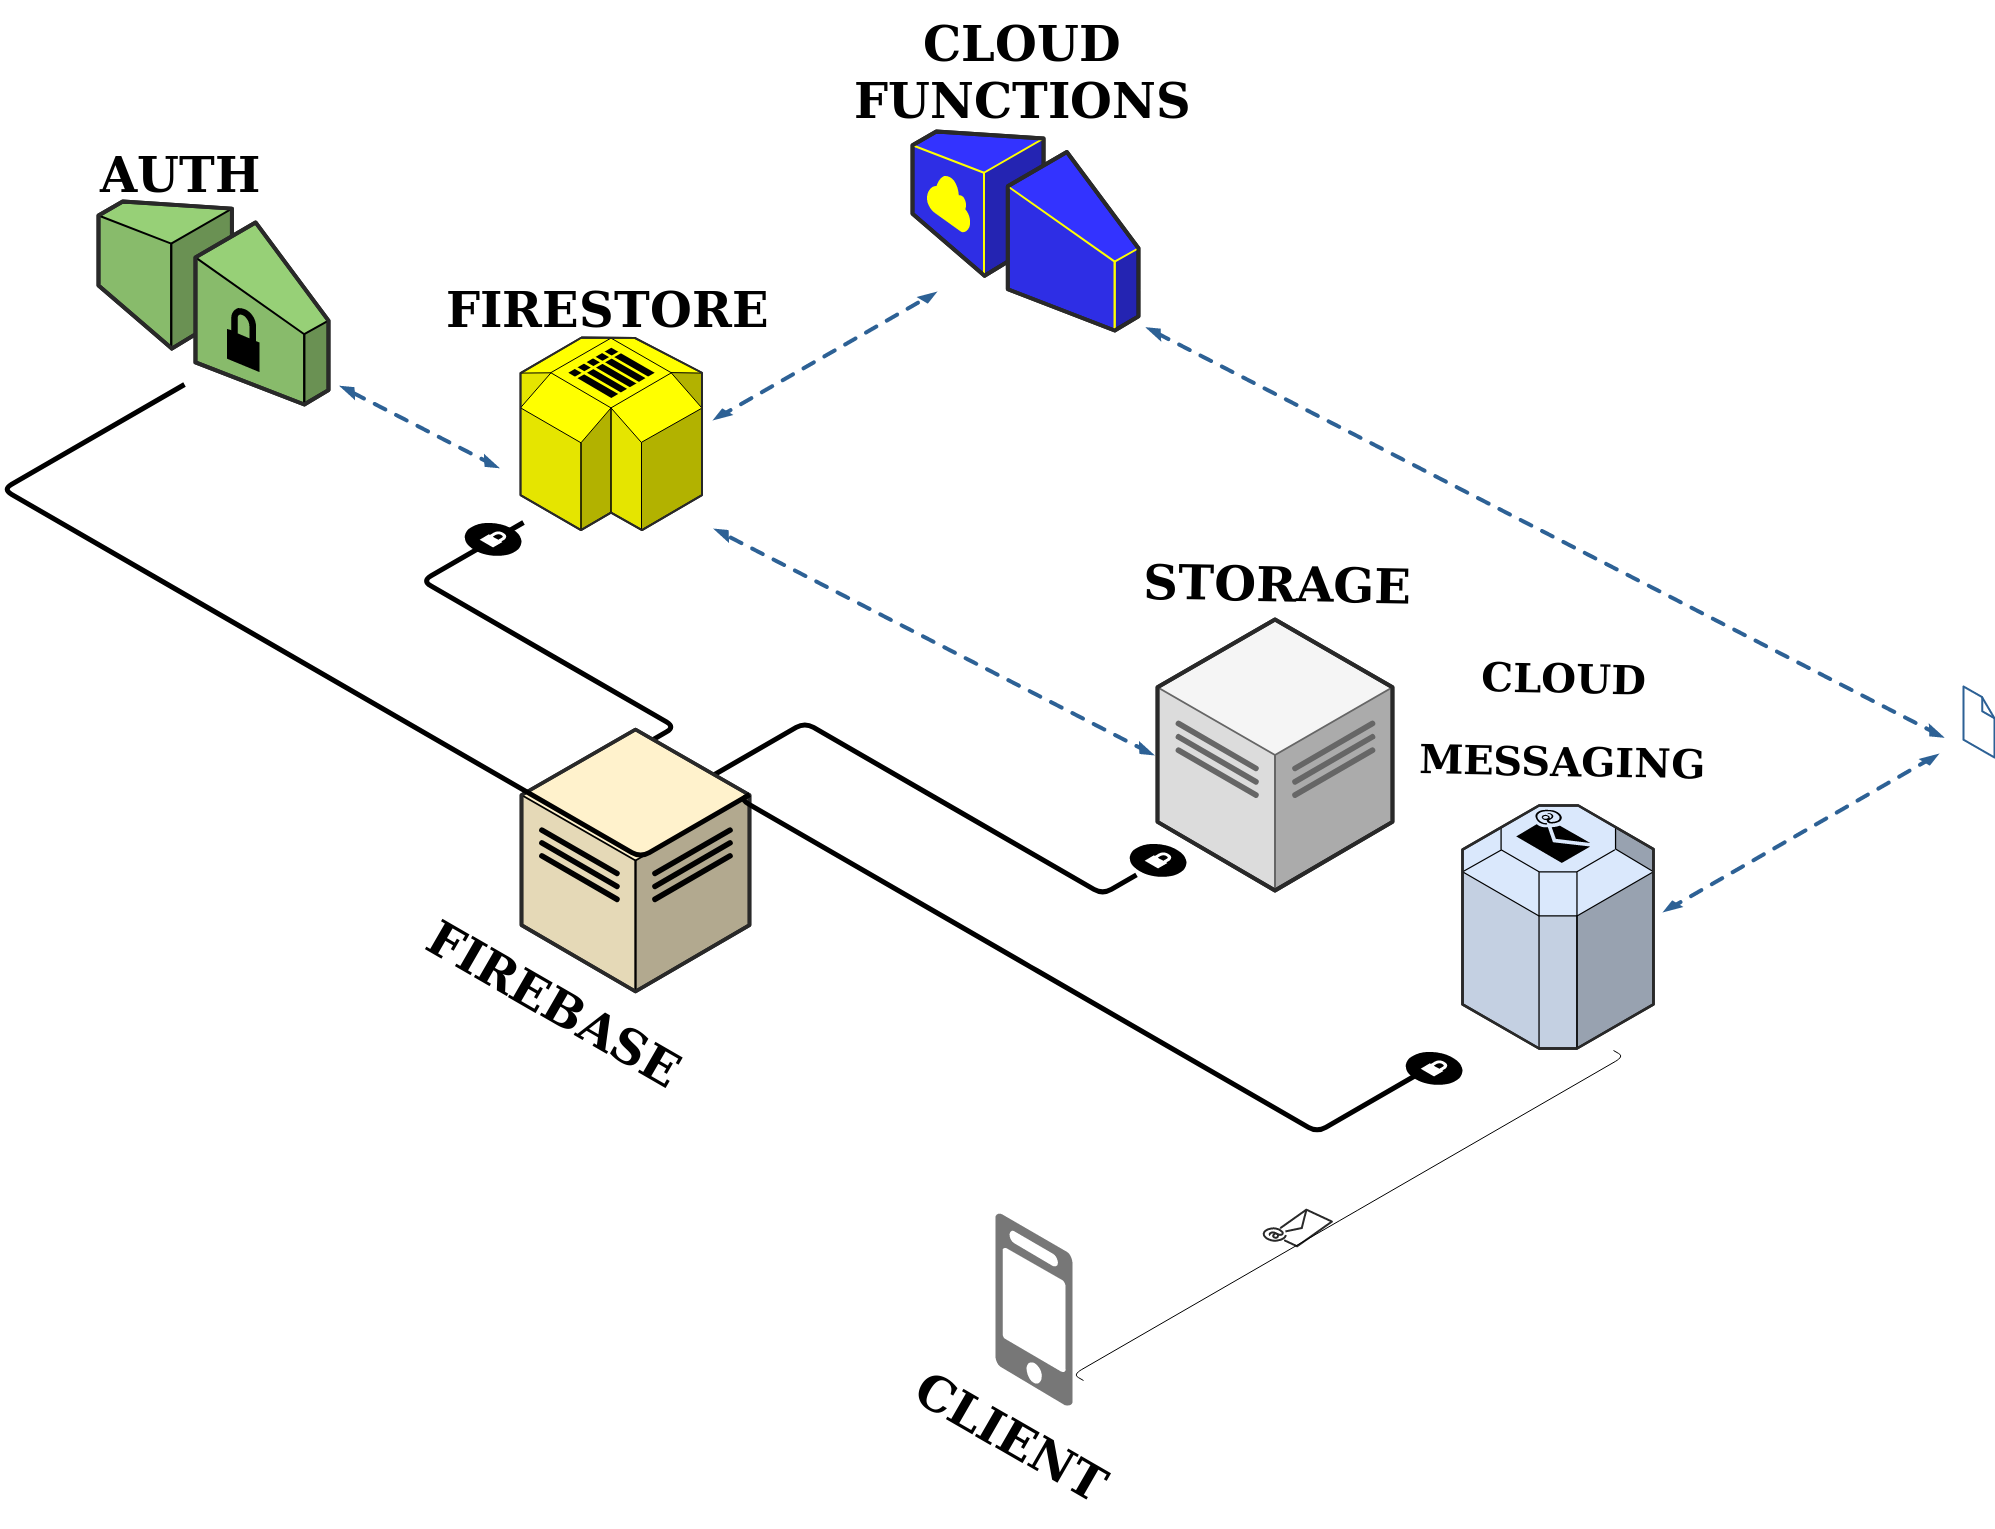
\includegraphics[width=0.7\textwidth]{immagini/server_arch.png}
  \caption{Server Architettura}\label{fig:Architettura Server}
\end{figure}


\section{Model View Presenter}                 %crea la sezione
MVP (Model View Presenter) \'e un pattern architetturale utilizzato per l'organizzazione strutturale di un progetto, in modo da trarne vantaggio in termini di prestazioni, leggibilit\'a e modularit\'a del codice.\\
La sua caratteristica principale \'e quella di separare il livello di presentazione dalla logica, in modo che tutto ci\'o che riguarda l'interazione dell'utente con l'interfaccia sia separato da come vengono rappresentati i dati.\\
Il pattern MVP deriva dal pattern MVC (Model View Controller), che ha 3 concetti base, che lo definiscono:

\begin{enumerate}
\item Model: Il modello dei dati da visualizzare
\item View: L'interfaccia utente che visualizza i dati
\item Controller: Controlla l'interazione tra Model e View
\end{enumerate}

La principale differenza tra i due pattern \'e che il Presenter del MVP gestisce la logica tra la View e il Model, e la sua implementazione permette di gestire l'interfaccia utente ma soprattutto rendere pi\'u comoda l'interazione tra interfaccia utente e i dati.\\


Come il pattern MVC, anche il pattern MVP permette di rendere le View indipendenti dalla gestione dei dati, dividendo la logica dell' applicazione in tre livelli distinti, livelli che possono essere testati separatamente.\\
La possibilit\'a di poter testare i livelli separatamente \'e una delle caratteristiche del MVP.\@


\begin{enumerate}
\item Model: Il modello \'e un' interfaccia che definisce i dati da visualizzare.
\item View: La View \'e un' interfaccia passiva che visualizza i dati (il modello) e instrada i comandi utente (eventi) al Presenter per agire su tali dati.
\item Presenter: Il Presenter agisce sul modello e sulla vista. Recupera i dati dai repository (il modello) e li formatta per la visualizzazione nella vista.
\end{enumerate}

\begin{figure}[!h]
  \centering
  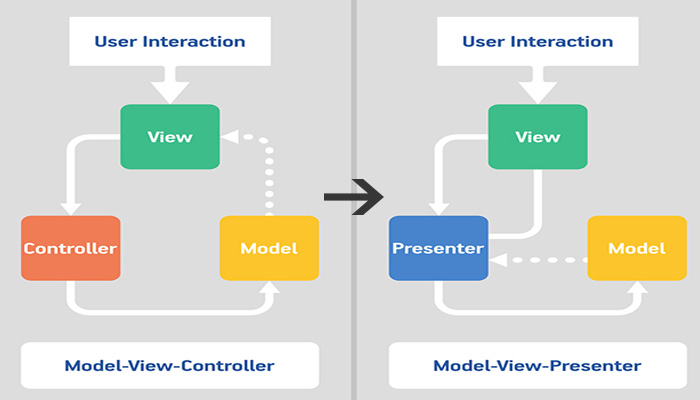
\includegraphics[width=0.65\textwidth]{immagini/mvc-vs-mvp.jpg}
  \caption{MVC vs MVP.}\label{fig:MVC vs MVP}
\end{figure}

\newpage


\subsection{Model}
Il Model \'e un'interfaccia dedicata all'acceso dei dati di un'applicazione, si occupa quindi di fornire un'astrazione del modello dei dati presenti nel database.\\
Il Model oltre a contenere la struttura dei dati da visualizzare si occupa anche di fornire una buona astrazione dei dati presenti nel database, modificando, aggiungendo e separando alcuni dei dati, in modo da rendere l'accesso e la visualizzazione dei dati pi\'u semplice per gli altri due componenti del pattern (View, Presenter).\\
Un esempio potrebbe essere il seguente:
Il database contiene una tabella con due tipi di dato:

\begin{enumerate}
\item \textbf{Nome}: String
\item \textbf{DataDiNascita}: Date
\end{enumerate}

Quando il programma ricever\'a i dati dal database in un qualsiasi formato( Map, Json, Array..) il Model selezionerà i dati in base alla definizione data dal programmatore trasformando il risultato del database in un oggetto.
Questo oggetto oltre a conserare le due informazioni ricevute dal database (Nome, DataDiNascita) potr'\a contenere ance informazioni aggiuntive inserite dal Model per facilitare l'uso e la manipolazione degli altri due componeti.
In questo caso il modello potrebbe creare il nuovo campo "et\'a" facendo una semplice sottrazione fra due date, quella attuale e la data di nascita dell'utente.

\begin{enumerate}
\item \textbf{Nome}: String
\item \textbf{DataDiNascita}: Date
\item \textbf{Et\'a}: Int
\end{enumerate}

%https://medium.com/@cervonefrancesco/model-view-presenter-android-guidelines-94970b430ddf

\subsection{View}
La View \'e un' interfaccia che definisce cosa deve implementare il Presenter, affinch\'e possa interagire con l'interfaccia utente.\\
La View interagisce con il Presenter per visualizzare i dati e notifica al Presenter le azioni che compie l'utente nell'interfaccia.\\
La View pu\'o essere implementata da un Activity, un Fragment, o un widget Android, che contengono ProgressBar, TextView, RecyclerView o altri elementi che necessitano di essere aggiornarnati in base a qualche azione dell'utente o cambiamento nel server.\\
Una delle problematiche riscontrare durante il testing delle view in Android sono causate della complessità del framework.Per risolvere questo problema, attraverso l'utilizzo del pattern MVP è possibile implementare una Passive View( modello di vista passivo).
La sua implementazione riduce al minimo la quantità di logica implementata nella vista.
Ad esempio, se si dispone di un modulo username/password e di un pulsante "Invia", non si scrive la logica di validazione all' interno della View ma all' interno del Presenter. La View infatti dovrebbe solo contenere il nome utente e la password e inviarli al Presenter.



\subsection{Presenter}
Il Presenter \'e il mediatore tra il Model e la View e si occupa di  recuperare i dati dal Model, formattarli e passarli alla View, ma a differenza del pattern MVC, decide anche cosa succede quando si interagisce con la View reagendo alle interazioni dell'utente.\\
Il Presenter per facilitare il testing deve cercare di non dipendere minimamente da Android, ma contenere solo metodi e dipendente Java, senza l'utilizzo del "Context" ad esempio, questo permetter\'a di scrivere i test per il Presenter senza l'utilizzo di un emulatore Android.\\
Come detto in precedenza  il Presenter deve dipendere dall' interfaccia View e non direttamente dall' Activity o Fragment, in questo modo si tengono separati il Presenter e l'Activity rispettando la D dei principi SOLID:"Dipendi dalle astensioni. Non dipendere dalle concrezioni"\\





%%%%%%%%%%%%%%%%%%%%%%%%%%%%%%%%%%%%%%%%%non numera l'ultima pagina sinistra
\clearpage{\pagestyle{empty}\cleardoublepage}

 \chapter{Sviluppo Client}                %crea il capitolo
%%%%%%%%%%%%%%%%%%%%%%%%%%%%%%%%%%%%%%%%%imposta l'intestazione di pagina
\lhead[\fancyplain{}{\bfseries\thepage}]{\fancyplain{}{\bfseries\rightmark}}

Inizialmente per sviluppare l'applicazione, è stato preso in considerazione il linguaggio Java, successivamente dopo aver testato le funzionalità di Java fu preso in considerazione Kotlin come linguaggio di programmazione per Android, in alternativa a Java, in modo tale da ricavare un confronto fra i due linguaggi.\\
In questo capitolo vengono illustrate e commentate le scelte implementative, l'organizzazione e la struttura utilizzata per organizzare i file in base al loro utilizzo.
L'applicazione è stata realizzata e sviluppata seguendo il pattern MVP, alcuni elementi di programmazione reattiva, cercando di rendere lo sviluppo di tutte le componenti dell'applicazione modulari e facili da gestire.



\newpage

\section{Struttura}
Il Client è stato strutturato in modo da contenere in packages differenti i componenti principali dell'applicazione.
\begin{itemize}
    \item \textbf{Pages:} Contiene quattro packages corrispondenti alle 4 funzionalità dell'app.
    \item \textbf{Activities:} Contiene le Actvity utilizzate dall'applicazione.
    \item \textbf{Models:} Contiene i modelli, utili per il pattern MVP
    \item \textbf{Repositories:} Contiene classi che facilitano la gestione e le richieste con il database.
    \item \textbf{Services:} Contiene due servizi per la gestione delle notifiche.
    \item \textbf{Utils:} Contiene classi utili per la gestione della cache, PreferenceShared e componenti view personalizzati.
\end{itemize}


\subsection{Pages}
L'implementazione delle funzionalità principali dell'applicazione sono contenute all'interno del package ``Pages'', ogni pagina rappresentante una funzionalità rispetta una logica comune per gestire l'interazione con l'utente e l'aggiornamento dei dati.\\
La logica utilizzata si basa sul pattern MVP, di conseguenza ogni volta che bisognerà mostrare dei dati, verranno implementati i seguenti componenti:
\begin{itemize}
    \item  \textbf{Adapter:} Estensione della classe "RecyclerView.Adapter" che contiene la lista elementi da visualizzare
    \item  \textbf{Presenter:} Componente che ha il compito di richiedere al Repository i dati da visualizzare
    \item  \textbf{View:} Interfaccia grafica della pagina con cui l'utente può interagire
    \item  \textbf{Model:} Modello astratto da rappresentare nella View
    \item  \textbf{Repository:} Classe che ha il compito di inviare richieste al Database, o di restituire le query necessarie per la richiesta al database
\end{itemize}
Le quattro pagine verranno illustrate e commentate nel dettaglio nell'apposita sezione del capitolo quattro.

\subsection{Activities}

Le Activity utilizzate dall'applicazione sono sette:
\begin{itemize}
  \item \textbf{BaseActivity:} gestisce il funzionamento dei menù (Menu delle impostazioni, Menù delle funzionalità), e si occupa di mostrare le quattro pagine principali
  \item \textbf{IntroActivity:} mostra delle pagine di introduzione all'applicazione, priama di poter effetuare, l'accesso o la registrazione
  \item \textbf{ProfileActivity:} mostra le informazioni personali dell'utente, e i campi che può modificare
  \item \textbf{GroupActivity:} mostra le informazioni del gruppo
  \item \textbf{JoinGroupActivity:} gestisce l'accesso ad un nuovo gruppo
  \item \textbf{NewGroupActivity:} gestisce la creazione di un nuovo gruppo
  \item \textbf{AuthActivity:} gestisce la logica dell'accesso e della registrazione

\end{itemize}

\subsubsection{Gestione gruppo}
La creazione e l'accesso ad un gruppo vengono gestite dalle activity ``JoinGroupActivity'' e ``NewGroupActivity''.\\
Effettuata la registrazione o l'accesso all'applicazione, l'utente avrà la possibilità di entrare a far parte di un gruppo o crearne uno nuovo, con l'eccezione che ogni utente può fare parte di un solo gruppo.\\
L'utente che sceglie di entrare a far parte di un nuovo gruppo deve aver precedentemente ricevuto il codice invito da un membro appartenente ad un gruppo esistente. Una volta ricevuto il codice di invito, il nuovo utente dovrà inserire il codice e confermare di entrare a far parte del gruppo, se conferma verranno aggiornati i membri del gruppo e il gruppo di appartenenza dell'utente e gli altri membri del gruppo invece riceveranno una notifica.\\
L'utente che sceglie invece di creare un nuovo gruppo deve indicare il nome del gruppo e un immagine opzionale da associarci, in seguito alla creazione potrà invitare altri utenti ad iscriversi al suo gruppo tramite un codice invito.

\subsubsection{Accesso e Registrazione}
Al primo avvio dell'applicazione, verranno mostrare delle pagine scorrevoli ``IntroActivity'' che illustreranno le caratteristiche principali con il quale può interagire l'utente, successivamente dopo una breve introduzione verrà mostrata la pagina di login, che permette di effettuare la registrazione e l'accesso attraverso un solo pulsante, senza differenziare se un utente sia già registrato o meno.\\
Quando l'utente cliccherà sul pulsane ``accedi'', l'applicazione automaticamente controllerà se l'utente si era già precedentemente registrato o deve effettuare la registrazione.\\
Se l'utente richiede di registrarsi, l'interfaccia e la logica di registrazione vengono controllate dalla libreria FirebaseUI, l'accesso invece viene gestito manualmente all'interno dell'activity ``AuthActivity''.\\
Ogni utente è univoco e non può creare account diversi utilizzando la stessa email, inoltre utilizzando la libreria FirebaseUI si hanno a disposizione l'integrazione con SmartLock, e l'account linking.
L'account linking consiste nel collegare account che utilizzano la stessa email, se si effettua, ad esempio l'accesso attraverso uno dei social supportati, e l'email di registrazione del social è già presente nei server di Firebase-Auth, verrà effettuato un collegamento degli account automatico (Account Linking), fra gli account che utilizzano la stessa email.\\
Quando un utente registrato, effettua l'accesso, viene controllato se è presente il record all'interno del database Firestore, in caso contrario viene fatta richiesta di aggiungere il nuovo utente al database Firestore, utilizzando come ID, l'identificativo fornito dal servizio Firebase-Auth. Una volta effettuato l'accesso per evitare ulteriori richieste al Database vengono anche salvate le informazioni dell'utente e gli identificativi dei membri appartenenti al gruppo nelle "Shared Preferences" di Android.\\
L'accesso e la registrazione possono essere effettuati utilizzando i social più diffusi o attraverso la semplice registrazione via email e password.\\
I social disponibili sono: Google, Facebook, Twitter

\begin{figure}[!hb]
  \centering
  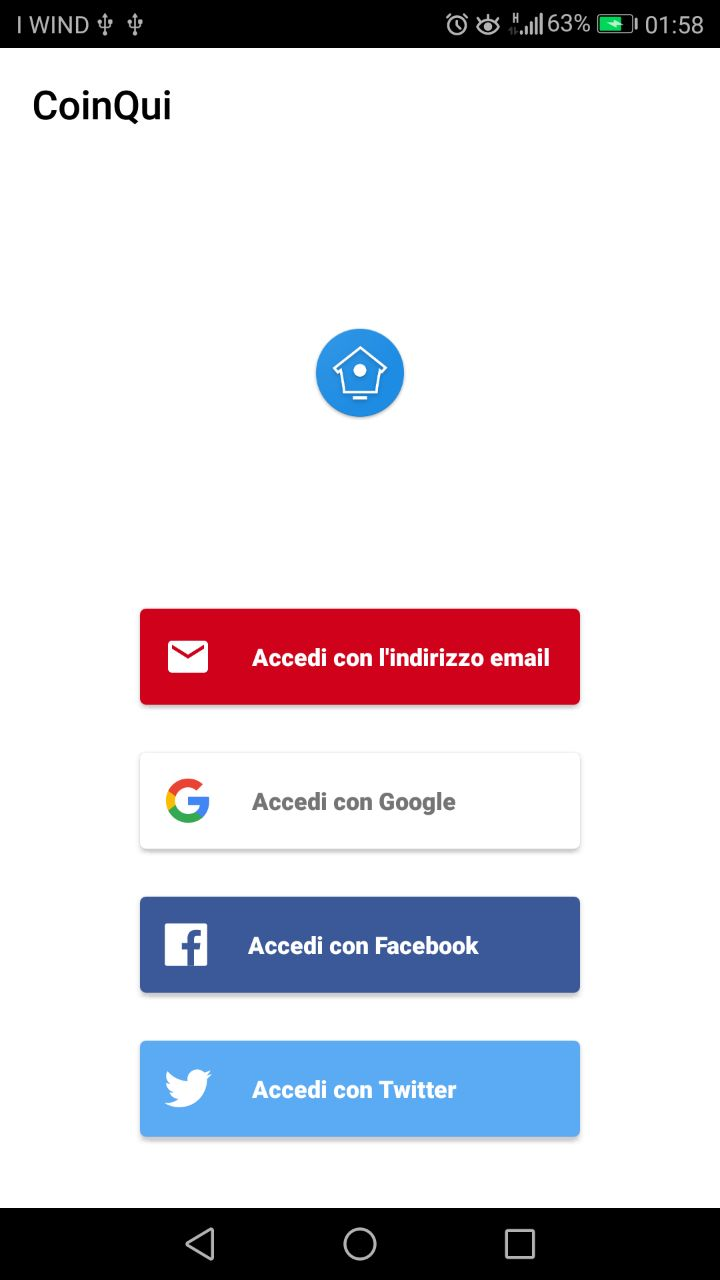
\includegraphics[width=0.3\textwidth]{immagini/app_login.jpg}
  \caption{Schermata applicazione Login}\label{fig:Schermata applicazione Login}
\end{figure}

Se l'utente sceglierà di registrarsi attraverso l'utilizzo di un email, gli verranno richiesti l'email di registrazione, un nominativo (Nome,Cognome) e una password, per effettuare il login invece verranno richiesti solo l'email e la password.\\
Alternativamente se l'utente seleziona il metodo di registrazione attraverso un social, comparirà a schermo una finestra che chiederà all'utente registrato al social di consentire l'utilizzo dell'email e del nome dell'utente da parte dell'applicazione, una volta ricevuta l'autorizzazione, le volte successive verrà effettuato un login automatico senza richiedere permessi aggiuntivi.\\
Un utente che ha dimenticato la propria password può richiederne una nuova inserendo l'email di registrazione, in seguito dopo pochi secondi riceverà via email un avviso per reimpostare la password e un link che permetterà di reimpostare la password.\\


\subsubsection{Menù}
L'applicazione offre due menù differenti, il menù delle funzionalità e il menù delle impostazioni, gestite dall'activity ``BaseActivity''.\\
Il menù delle funzionalità si trova nella parte inferiore dello schermo, mentre per accedere al menù delle impostazioni, bisognerà cliccare la relativa icona del menù presente nella toolbar.\\

\begin{figure}[!hb]
  \centering
  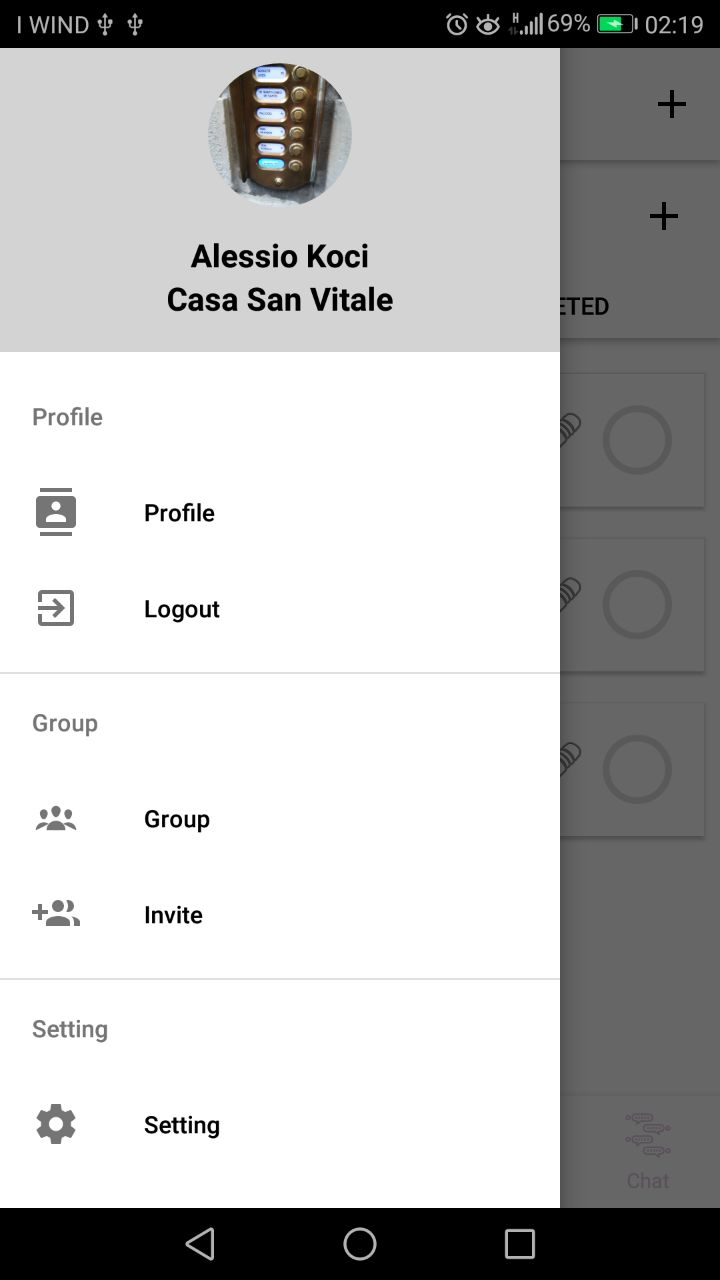
\includegraphics[width=0.3\textwidth]{immagini/app_menu.jpg}
  \caption{Schermata applicazione Menù}\label{fig:Schermata applicazione Menu}
\end{figure}

Interagendo con il menù delle impostazioni laterale si potranno gestire le informazioni personali dell'utente e gestire le informazioni del suo gruppo.\\
Nella pagina riguardante il profilo ``ProfileActivity'' dell'utente sarà possibile visualizzare le informazioni personali come il nome, l'email e il gruppo a cui esso appartiene, queste informazioni sono modificabili in qualsiasi momento.\\
Nella pagina riguardante il gruppo ``GroupActivity'' invece sarà possibile visualizzare le informazioni principali riguardanti il gruppo a cui l'utente appartiene, come: il nome, l'immagine e gli utente che appartengono al gruppo. Le informazioni modificabili in questa pagina sono l'immagine del gruppo, il nome del gruppo e la possibilità di invitare altre persone ad unirsi al gruppo tramite invito, (verrà inviato all'utente un codice di invito che dovrà inserire al momento della registrazione).\\



\subsection{Repository}
All'interno del package Repositories sono presenti le classi necessarie per interagire con il database Firestore.\\
Sono presenti due tipi di classi:
\begin{itemize}
    \item \textbf{Query:} Sono classi che contengono le query necessarie per interagire con il database, ogni classe conterrà le query relativa alle sue funzionalità, la funzione Todolist dell'applicazione ad esempio avrà una classe TodoListQuery.
    \item \textbf{Repository:} Sono classi che restituiscono un oggetto Single, Observable o Completable in base al tipo di richiesta effettuata. Ogni Repository richiamerà la relativa classe Query per ricevere l'istruzione necessaria per aggiungere modificare o richiedere dei dati al database.
\end{itemize}

Un esempio di una Repository è il seguente:

\begin{lstlisting}[language=kotlin,caption={Esempio RepositoryAggiunta elemento Todolist}]
fun getTodoItems(): Single<List<TodoItem>> {
       return Single.create<List<TodoItem>> { emitter ->
           queryTodo.getTodoItems().addSnapshotListener({ querySnapshot, exception ->
               if (exception != null)
                   emitter.onError(Throwable(exception))
               else {
                   emitter.onSuccess(TodoItem.mapping(querySnapshot))
               }
           })
       }
   }
\end{lstlisting}
Ogni Repository non conosce la query necessaria per effettuare la richiesta al database ma utilizzando la rispettiva classe che restituisce la query necessaria per richiedere al database la lista degli elementi all'interno della todolist.



\subsection{Utils}
Il package Utils contiene classi di supporto per azioni comuni che vengono svolte dai componenti dell'applicazione.\\
In particolare le principali sono:
\begin{itemize}
    \item \textbf{PreferenceUtils:} Classe utilizzata per gestire le SharedPreferences.
    \item \textbf{ImageUtils:} Classe che interagendo con la libreria Glide, aggiunge funzionalità alla gestione delle immagini.
    \item \textbf{RxFirestore:} Estensioni effettuate su alcuni oggetti dell'SDK Firestore per implementare il pattern Observable.
    \item \textbf{UserSpinner:} Componente View che estende. AppCompatSpinner, creato per mostrare e selezionare graficamente gli utenti attraverso uno spinner.
    \item \textbf{FirestoreCMUtils:} Classe che gestire i Token utilizzati da Cloud Messaging.
\end{itemize}

La classe PreferenceUtils memorizza le informazioni riguardanti gli utenti apparteneti al gruppo, le informazioni personali dell'utente consentendo di modificarne i valori e cancellare tutti i dati e le cache dell'applicazione.\\.
La classe ImageUtils, è stata realizzata per estendere alcune funzionalità della libreria Glide, utilizzata per visualizzare le immagini, in particolare è stato implementato un metodo per visualizzare un immagine attraverso un link URL. La libreria opportunamente modificata consentiva di scarichere l'immagine del link, memorizzarla nella cache e renderla visibile all'utente attraverso l'interfaccia.\\
Il file RxFirestore contiene le funzioni necessarie per implementare dei metodi aggiuntivi agli oggetti DocumentReference, CollectionReference messi a disposizione dall'SDK di Firebase per fare riferimento ad una collezione o documento all'interno del database. I metodi aggiuntivi consentono di applicare la programmazione reattiva alle chiamate eseguite per richiedere e modificare dati all'interno del database Firestore.
UserSpinner è un widget creato appositamente per mostrare una finestra di dialogo contenente la lista del nome degli utenti appartenenti al gruppo, e una checkbox per ogni utente, offrendo quindi la possibilità di selezionare uno o più utenti durante la creazione di una nuova mansione, spesa o evento.\\
Infine la classe FirestoreCMUtils gestisce i token e i gruppi associati ad un token di Cloud Messaging, la classe in particolare viene utilizzata per generare un token necessario per connettersi ai server FCM, creare un nuovo gruppo di utenti indicando i token di ogni dispositivo, e per ultimo gestire l'aggiunta di un nuovo utente ad un gruppo di utenti preesistenti.

\subsection{Modelli}
I modelli sono stati realizzati utilizzando le data class offerte da Kotlin, in questo modo non è stato necessario implementare i metodi get e set come quando si devono creare dei modelli in Java. L'unica aggiunta effettuata è stata la creazione di due nuovi metodi chiamati "mapping" che permettono di convertire i tipi DocumentSnapshot e QuerySnapshot restituiti dal'SDK Firebase come risposta ad una richiesta effettuata al database Firestore in modelli utilizzabili come oggetti all'interno dell'applicazione, mappando quindi ogni valore contenuto negli SnapShot all'interno dei singoli valori del modello.\\
I modelli vengono utilizzati nell'applicazione per rispettare il pattern MPV garantendo una buona interazione dei dati con l'interfaccia grafica, e soprattutto per avere una migliore gestione dei tipi durante la chiamata e la restituzione di valori associati ad una funzione.\\
Un esempio di un modello utilizzato è il seguente:
\begin{lstlisting}[language=kotlin,caption={Aggiunta elemento Todolist}]

data class GroupItem(
        var id: String = "",
        var name: String? = null,
        var creation_date: Date = Date(),
        var logo: String? = null,
        var users: Map<String, Boolean> = emptyMap(),
        var tokenFCM: String? = null
)
\end{lstlisting}
Il seguente modello rappresenta un documento all'interno della collezione contenente i gruppi. Attraverso il costrutto data class, e inizializzando le variabili con la keyword ``var'' Kotlin in automatico in fase di compilazione aggiungerà i metodo necessari per settare e ricevere i valori dalla classe GroupItem.\\
L'id di ogni gruppo è impostato come stringa vuota, e verrà settato al momento dell'aggiunta di un nuovo gruppo, come il nome il logo e la lista degli utenti.\\
Il valore ``data'' è assegnato di default in base alla data di creazione del gruppo, mentre il tokenFCM è generato subito dopo la creazione del gruppo, attraverso il servizio FCM.

\subsection{Servizi}
I servizi utilizzati dall'applicazione sono stati creati per interagire con il servizio Cloud Messaging di Firebase.\\
I servizi sono due:
\begin{itemize}
    \item \textbf{FirebaseMessagingService}
    \item \textbf{FirebaseInstanceIdService}
\end{itemize}

Il primo: FirebaseMessagingIdService gestisce i token necessari per utilizzare Cloud Messaging, in particolare gestisce l'aggiornamento del token del dispositivo, inviando una richiesta di aggiornamento al Database Firestore, qualora il token sia aggiornato o eliminato.\\
Il secondo servizio invece: FirebaseInstanceService gestisce i messaggi ricevuto dal server di Cloud Messaging, implementando il metodo ``onMessageReceived'' sarà possibile innanzitutto capire il tipo di messaggio ricevuto da FCM (messaggio di notifica o messaggio contenente dati), successivamente in base al tipo di messaggio ricevuto vengono effettuate modifiche o mostrate le adeguate notifiche.\\
Oltre ad aggiungere la libreria che si occupa di interagire con il servizio FCM, è stato necessario indicare all'interno del AndroidManifest del progetto, che le due classi create sono dei servizi:
\begin{lstlisting}[language=kotlin,caption={Android Manifest - I servizi FCM}]
<service android:name=".Services.FirestoreEventFunctionService">
           <intent-filter>
               <action android:name="com.google.firebase.MESSAGING_EVENT" />
           </intent-filter>
       </service>
       <service android:name=".Services.FirestoreEventFunctionnstanceIDService">
           <intent-filter>
               <action android:name="com.google.firebase.INSTANCE_ID_EVENT" />
           </intent-filter>
       </service>
       \end{lstlisting}
In particolare quando viene ricevuto il messaggio di aggiunta di un nuovo membro nel gruppo, oltre ad inviare la notifica per avvisare i dispositivi, vengono anche aggiornate le PreferenceShared che contiene localmente una copia delle informazioni riguardanti il gruppo senza dover contattare ripetutamente il database.\\

\begin{lstlisting}[language=kotlin,caption={Metodo onMessageReceived}]

override fun onMessageReceived(remoteMessage: RemoteMessage ? ) {
...
  val msgData = remoteMessage.data.toProperties()
  val loggedUser = PreferenceUtils(context = applicationContext).getUserUID()
  if (remoteMessage.data.isNotEmpty()) {
   val msgData = remoteMessage.data.toProperties()
   val loggedUser = PreferenceUtils(context = applicationContext).getUserUID()
   if (msgData.getProperty("sender") != loggedUser) {
    when(msgData.getProperty("type")) {
      ...
     "todo" -> {
      sendNotification(messageTitle = R.String.new_todo_item, messageBody = msgData.getProperty("name"))
     }
     ...
    }
   }
  }
}
\end{lstlisting}
La funzione "onMessageReceived" viene richiamata quando il server FCM segnala al dispositivo la ricezione di un nuovo messaggio. Successivamente, verrà controllato se l'utente, che ha compiuto il cambiamento all'interno del database, aggiungendo o modificando un elemento, è lo stesso utente loggato all'interno dell'applicazione, in caso affermativo non verrà inviata nessuna notifica al dispositivo, in caso contrario verrà mostrata una notifica, avvisando l'utente del nuovo cambiamento all'interno dell'applicazione.

\section{Funzionalità}
L'applicazione aiuta la gestione di attività e problemi riscontrati durante una convivenza fra due o più persone, in ambito lavorativo o fra studenti fuori-sede.\\
Le funzionalità principali consentono ai membri di un gruppo di gestire una lista di mansioni comuni da svolgere, gestire e dividere le spese, organizzare eventi periodici e/o ricorrenti e confrontarsi utilizzando la chat di messaggistica istantanea.
L'applicazione avendo funzionalità molto generiche lascia il completo utilizzo di esse all'utente finale, permettendogli di gestire le varie funzionalità come meglio crede. Un esempio potrebbe essere la gestione degli eventi: alcuni studenti fuori sede potrebbero creare eventi per organizzare i turni di pulizia all'interno della casa, assegnando eventi ricorrenti a coinquilini specifici, in ambito lavorativo invece, i membri del gruppo potrebbero utilizzare la funzione di gestione degli eventi per organizzarsi il lavoro o creare incontri aziendali.\\
L'utente dopo aver effettuato l'accesso potrà interagire con le funzionalità dell'applicazione selezionando l'icona della relativa funzionalità dal menù.
La struttura e l'organizzazione dei file delle quattro funzionalità dell'app è la stessa, inoltre il pattern utilizzato per la gestione fra le varie componenti del progetto per interagire con i dati e l'interfaccia utente è MVP (Model View Presenter).\\
Esiste una Activity principale chiamato BaseActivity che gestisce il funzionamento dei menù (Menu delle impostazioni, Menù delle funzionalità), e si occupa di mostrare le quattro pagine principali, realizzate estendendo la class Fragment.\\
I quattro Fragment sono quindi:
\begin{itemize}
    \item \textbf{FragmentTodo:} Pagina per visualizzare e interfacciarsi con le mansioni del gruppo
    \item \textbf{FragmentSpese:} Pagina per visualizzare e interfacciarsi con le spese del gruppo
    \item \textbf{FragmentEventi:} Pagina per visualizzaere e gestire gli eventi del gruppo
    \item \textbf{FragmentChat:} Pagina per accedere alla chat di messaggistica istantanea del gruppo
\end{itemize}
I fragment vengono cambiati e gestiti dall'Activity principale, che in base all'interazione con il menu delle funzionalità, si interscambiano.
\begin{lstlisting}[language=kotlin,caption={Aggiornamento fragment del BaseActivity}]
 supportFragmentManager.beginTransaction().replace(R.id.activity_content, TodoFragment()).commit()
\end{lstlisting}

Quando si seleziona una della pagine, il controllo dell'interfaccia passa al relativo Fragment, che in base alla funzionalità mostrerà e permetterà di agire sull'interfaccia.

\newpage
\subsection{Todolist}

Selezionando dal menù dell'applicazione l'icona della ``Todolist'', l'utente visualizzerà l'interfaccia dedicata per interagire con le funzionalità della todolist, quali: visualizzare le mansioni da svolgere, visualizzare le mansioni già svolte, aggiungere, modificare o eliminare una mansione.\\
L'interfaccia per visualizzare le mansioni è composta da due sezioni, la sezione delle mansioni da completare, in primo piano e le mansioni già completate in un'apposita sezione.\\
Le mansioni sono composte da un nome obbligatorio, una data di scadenza, una priorità ed i membri del gruppo a cui è rivolta la mansione.\\
Ogni utente visualizza la mansione comprensiva di nome e data, la priorità invece viene indicata con un bordo colorato in base all'importanza della mansione, le altre informazioni possono essere viste, cliccando sulla mansione.\\

\begin{figure}[!hb]
  \centering
  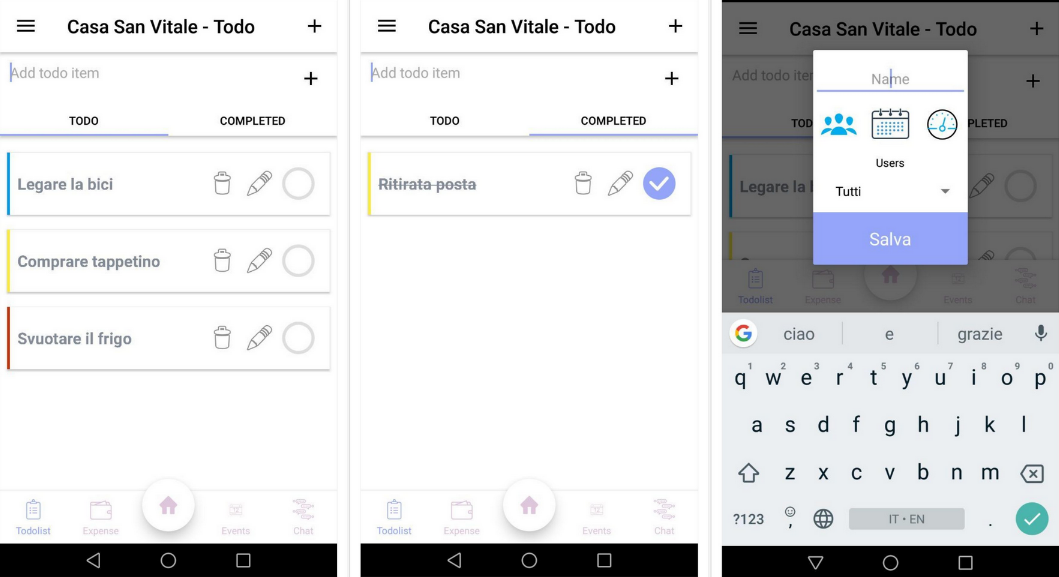
\includegraphics[width=0.85\textwidth]{immagini/app_todolist.png}
  \caption{Schermata applicazione Todolist}\label{fig:Schermata applicazione Todolist}
\end{figure}


Gli utenti possono vedere sia le mansioni create dagli altri membri del gruppo sia le loro mansioni, in base alle restrizioni di visibilità assegnate durante la creazione, l'unica limitazione imposta riguarda le funzionalità di modifica ed eliminazione, che sono consentite solamente all'utente che ha creato la mansione, gli altri utenti invece potranno completare la mansione marcandola.\\
Le mansioni che vengono marcate e completate vengono spostate automaticamente nell'elenco delle mansioni completate e ogni utente avrà la possibilità di portare nuovamente una mansione non completata nella sezione delle mansioni da completare, senza dover aggiungerne un'ulteriore. Quando si sposta una mansione dalla sezione ``mansioni completate'' alla sezione ``mansioni da completare'' il nome, la visibilità e la priorità della mansione rimarranno inalterate, mentre la data di scadenza sarà impostata al giorno in cui è avvenuto il cambiamento.\\
L'aggiunta di una nuova mansione viene effettuata attraverso due modalità differenti: la prima rapida, la seconda personalizzata.\\
La modalità rapida si trova nella parte superiore dello schermo, sottostante alla toolbar, in questa modalità l'utente può aggiungere un nuovo elemento indicando solamente il nome ed in automatico l'applicazione setterà i campi opzionali, impostando la data di scadenza alla data in cui è stato aggiunto l'elemento, la priorità di medio livello e la visibilità a tutti i membri del gruppo.\\
La modalità personalizzata invece permette di inserire tutte le informazioni possibili per una mansione, questa modalità di aggiunta compare se l'utente clicca la relativa icona presente nella toolbar della pagina "Todolist". Una volta cliccata l'icona si aprirà una finestra con un testo da completare corrispondente al nome della mansione e tre icone: l'icona di una data, l'icona di un gruppo e l'icona della priorità, che se cliccate consentono all'utente di inserire le informazioni opzionali.
\begin{itemize}
    \item \textbf{Priorità:} la priorità di una mansione dispone di 3 opzioni:``Bassa priorità'', ``Alta priorità'' e ``Media priorità''.
    \item \textbf{Visibilità:} la visibilità di una mansione si potrà indicare selezionando da una lista gli utenti del gruppo.
    \item \textbf{Data:} la data viene impostata, attraverso un calendario, indicando il giorno di scadenza della mansione.
\end{itemize}



Il fragment TodolistPage, si occupa di gestire l'aggiunta rapida di un nuovo elemento e la logica delle due Tab "Da completare" "Completato".\\
L'aggiunta di un elemento con la modalità rapida, inserendo solamente il nome della mansione, viene svolta, inizializzando un nuovo elemento di tipo Todolist, contenente il nome inserito dall'utente e impostando i valori di default della mansione.\\ Successivamente viene inizilizzata la Repository che ha il compito di gestire l'interazione con il database per la lista delle mansioni, attraverso un approccio asincrono, il fragment attenderà la risposta dal Database e in caso negativo mostrerà un errore.

\begin{lstlisting}[language=kotlin,caption={Aggiunta elemento Todolist}]
val todoItem = TodoItem(name = itemName, date = Date(), members = members, created_by = userUID)
todoRepo.add(todoitem = todoItem).observeOn(AndroidSchedulers.mainThread()) .subscribeOn(Schedulers.io()).doOnComplete {
    todolist_editext_newitem.setText("")
    Toast.makeText(context, "todoitem successfully created!", Toast.LENGTH_SHORT).show()
}.doOnError {
            Toast.makeText(context, "error!", Toast.LENGTH_SHORT).show()
        }.subscribe()
\end{lstlisting}

Il componente TabLayout che mostra le due Tab richiede l'utilizzo di un Adapter che estende la class FragmentStatePagerAdapter, in questo modo quando un utente interagirà con una delle due Tab, l'Adapter si occuperà di istanziare il Fragment corrispondente per visualizzare la lista delle mansioni completate o non completate.\\
Dato che per visualizzare gli elementi completati e da completare, teoricamente sarebbero servite due Fragment con parti di codice molto simile, si è scelto di realizzarne solamente uno, che in base al valore di un parametro chiamato ``type'', passato nella creazione dell'istanza del fragment, visualizzerà elementi differenti.\\

\begin{lstlisting}[language=kotlin,caption={FragmentTodo.kt}]
companion object {
       fun newInstance(type: Int): TodoFragment {
           val fragment = TodoFragment()
           fragment.type = type
           return fragment
       }
   }
\end{lstlisting}
\subsection{Spese}
La seconda funzionalità principale dell'applicazione è la gestione delle spese condivise, per accedere a questa funzionalità l'utente dovrà cliccare l'icona di un portafoglio dal relativo menù delle funzionalità.\\
L'interfaccia che si presenta all'utente è molto simile all'interfaccia della gestione delle mansioni: è presente la visualizzazione globale delle spese da pagare e pagate e la possibilità di aggiungerne modificarne o cancellarne una.\\
Ogni utente appartenente al gruppo visualizzerà tutte le spese non completate e quelle già completate e in qualsiasi momento potrà marcare una spesa, segnandola come pagata.\\
La visualizzazione dei una singola spesa comprende di nome, la data di scadenza, l'icona della categoria a cui è associata la spesa, e la quota parziale che dovrà pagare l'utente. Cliccando su una spesa apparirà una finestra di dialogo che mostrerà il resoconto totale della spesa con la lista degli utenti che hanno pagato la loro quota e la lista degli utenti che ancora devono pagarla. Marcando una spesa l'utente segnerà di aver pagato la sua quota e di conseguenza la spesa, per quell'utente, verrà spostate automaticamente nell'elenco delle spese pagate.\\

\begin{figure}[!h]
  \centering
  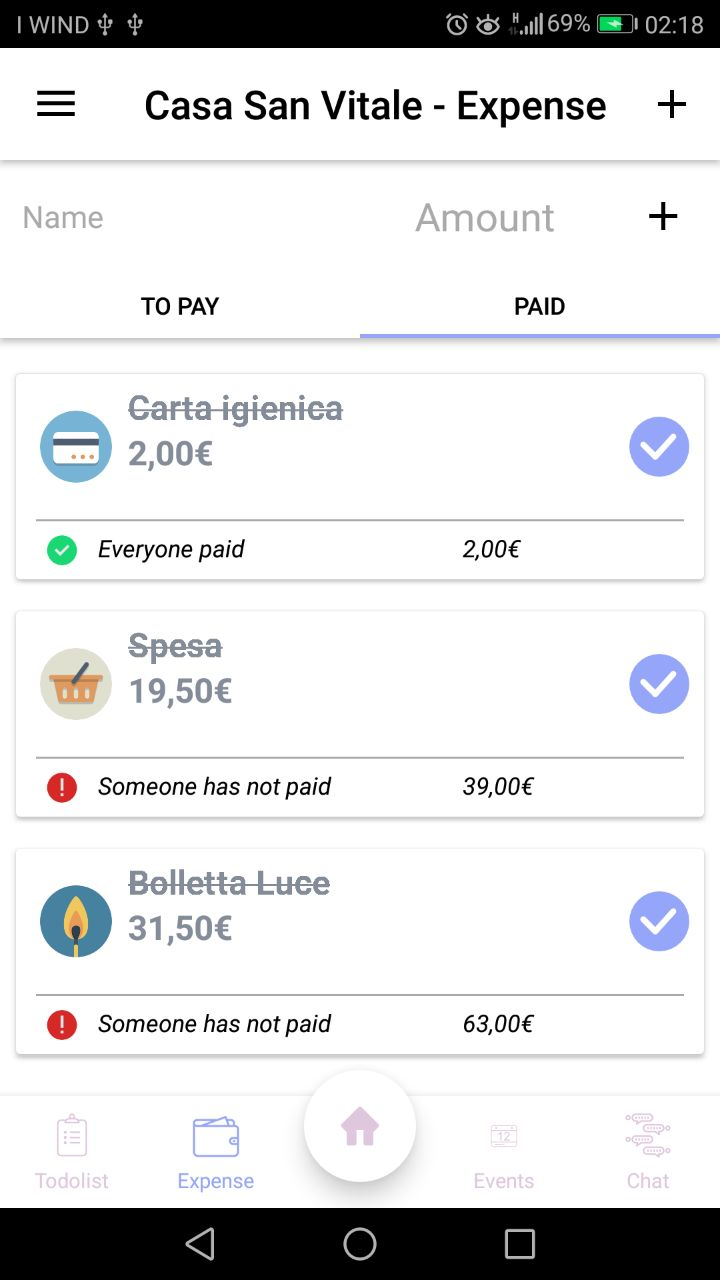
\includegraphics[width=0.3\textwidth]{immagini/app_expense.jpg}
  \caption{Schermata applicazione Spese}\label{fig:Schermata applicazione Spese}
\end{figure}

Le funzionalità di modifica ed eliminazione di una spesa sono consentite solamente all'utente che ha creato la spesa, gli altri utenti invece potranno solamente indicare di aver pagato la quota, marcandola.\\
Le modalità di aggiunta di una nuova spesa sono due, la modalità rapida e la modalità personalizzata.\\
La modalità rapida è accessibile attraverso l'interfaccia principale, nella parte superiore dello schermo infatti sono presenti due caselle di testo e un pulsante.Questa modalità permette di indicare solamente i parametri obbligatori: il nome e l'ammontare globale, alternativamente se l'utente vuole specificare anche altre informazioni, dovrà utilizzare il relativo pulsante per accedere alla finestra con tutti i campi opzionali per la creazione di una spesa.\\
La modalità di aggiunta personalizzata invece prevede un interfaccia con una casella di testo corrispondente al nome della spesa, e un'altra casella di testo corrispondente all'ammontare globale, sottostante alle caselle ci saranno tre icone: l'icona di un calendario, l'icona di un file, l'icona di un gruppo e l'icona di un etichetta, che se cliccate consentiranno all'utente di inserire le informazioni opzionali.

\begin{itemize}
   \item \textbf{Descrizione:} Casella di testo per indicare una descrizone della spesa
   \item \textbf{Visibilità:} Scelta multipla fra gli utenti del gruppo per indicare a chi è rivolta la spesa.
   \item \textbf{Data:} Calendario per indicare il giorno di scadenza della spesa.
   \item \textbf{Categoria:} Scelta multipla per indicare il la tipologia di spesa effettuata
\end{itemize}
Le categorie selezionabili sono preimpostate dall'applicazione e sono le seguenti:
\begin{itemize}
    \item Bolletta Gas
    \item Bolletta Acqua
    \item Bolletta Luce
    \item Bolletta Telefono
    \item Cibo
    \item Pulizie
    \item Casa
    \item Strumenti
    \item Spesa generica
\end{itemize}
L'implementazione di questa funzionalità utilizza sempre il pattern MPV e la logica e simile a quella della funzionalità TodoList.


\subsection{Eventi}
Un'altra funzionalità è la gestione degli eventi, che permetterà ai membri del gruppo di creare degli eventi indicando una data, e qualora l'evento fosse ricorrente indicando la ricorrenza dell'evento.\\
L'interfaccia della pagina dedicata agli eventi è molto semplice, sulla parte superiore della toolbar è presente un icona che permette di aggiungere un nuovo evento, sottostante ad essa sono presenti tutti gli eventi sottoforma di lista.\\
Quando un utente clicca sull'icona per inserire un nuovo evento, verrà mostrata una finestra di dialogo, dove l'utente dovrà indicare il nome dell'evento, un eventuale descrizione, i partecipanti all'evento, e la ricorrenza dell'evento. La ricorrenza dell'evento può essere di cinque tipi differenti:
\begin{itemize}
  \item Non ripetere
  \item Giornaliera
  \item Settimanale
  \item Mensile
  \item Annuale
\end{itemize}



Una volta selezionata la ricorrenza verrà richiesta la data di riferimento dell'evento.\\
Gli utenti hanno la possibilità di aggiungere all'interno del gruppo eventi classici ed eventi ricorrenti. La logica utilizzata per visualizzare ed aggiungere elementi all'interno del database è la stessa utilizzata per le precedenti funzionalità, è quindi presente un fragment principale, una view, un presenter che richiede al database firestore i dati da visualizzare, e un adapter.\\
Durante l'aggiunta di un nuovo elemento è stata usata la libreria SublimePicker che offre l'interefacia di un calendario personalizzabile, con cui far interagire l'utente per selezionare una data e impostare una ricorrenza. Il Widget SublimePicker necessita di un inizializzazione con il passaggio di un oggetto ``SublimeOptions'' per poter funzionare.\\

\begin{figure}[!h]
  \centering
  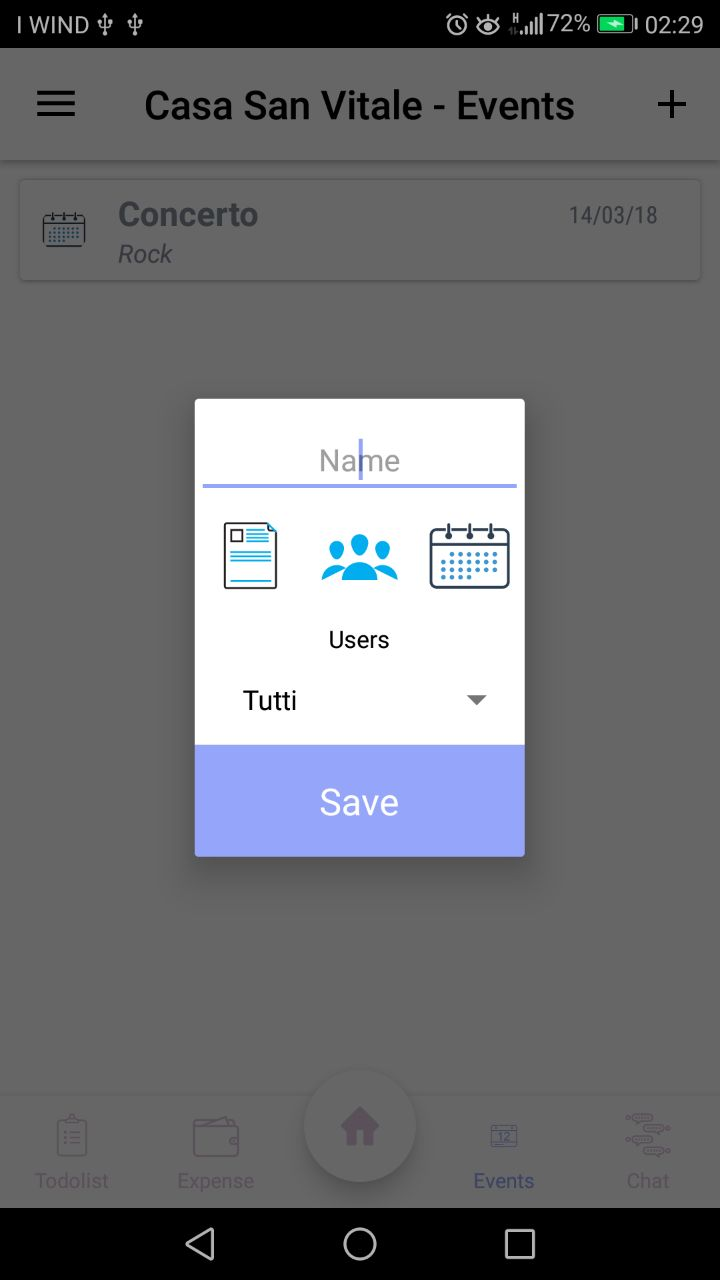
\includegraphics[width=0.3\textwidth]{immagini/app_event.jpg}
  \caption{Schermata applicazione Eventi}\label{fig:Schermata applicazione Eventi}
\end{figure}

\begin{lstlisting}[language=kotlin,caption={Configurazione del Widget SublimePicker}]
..
val options = SublimeOptions()
var displayOptions = 0
displayOptions = displayOptions or SublimeOptions.ACTIVATE_DATE_PICKER
displayOptions = displayOptions or SublimeOptions.ACTIVATE_RECURRENCE_PICKER
options.pickerToShow = SublimeOptions.Picker.REPEAT_OPTION_PICKER
options.setDisplayOptions(displayOptions)
options.setCanPickDateRange(false)
..

\end{lstlisting}
Una volta indicati i parametri di default del Widget sarà possibile renderlo disponibile graficamente all'utente.
Nella visualizzazione degli eventi per distingue se un evento è ricorrente è stato ricavato un nuovo dato non presente nel database, che consiste nel differenziare eventi ricorrenti da eventi che non hanno nessuna ricorrenza.\\

\begin{lstlisting}[language=kotlin,caption={Linea di codice del modello Event}]
   var is_recurring = result.getString("recurring_type").isNullOrBlank().not()
\end{lstlisting}

Gli eventi ricorrenti hanno assegnato il valore di ricorrenza (Dayly,Weekly,Monthly,Yearly) all'interno della variabile ``recurring'\_type'', di conseguenza effettuando un controllo sul contenuto della variabile è possibile creare la variabile booleana ``is'\_Recurring'' che differenzia i due tipi di eventi

\subsection{Chat}
L'interfaccia della sezione chat è simile ad altre applicazioni di messaggistica istantanea e consente di visualizzare tutti i messaggi inviati dall'utente e ricevuti dagli altri membri del gruppo.\\
I messaggi inviati dall'utente saranno contrassegnati con un colore blu e si troveranno nella parte destra dello schermo, mentre i messaggi ricevuto dagli altri membri del gruppo si troveranno nella parte sinistra dello schermo con un colore differente e informazioni aggiuntive come il nome e l'avatar dell'utente che ha inviato il messaggio.
Nella parte inferiore dello schermo è presente una casella di testo e un pulsante consentendo all'utente di scrivere e inviare un nuovo messaggio che sarà spedito in tempo reale a tutti i membri del gruppo, infatti una volta inviati, i messaggi appariranno come notifica a tutti i dispositivi online.\\
Quando un utente non dispone di una connessione internet, il messaggio verrà conservato e l'utente verrà notificato appena si connetterà ad internet.

\begin{figure}[!h]
  \centering
  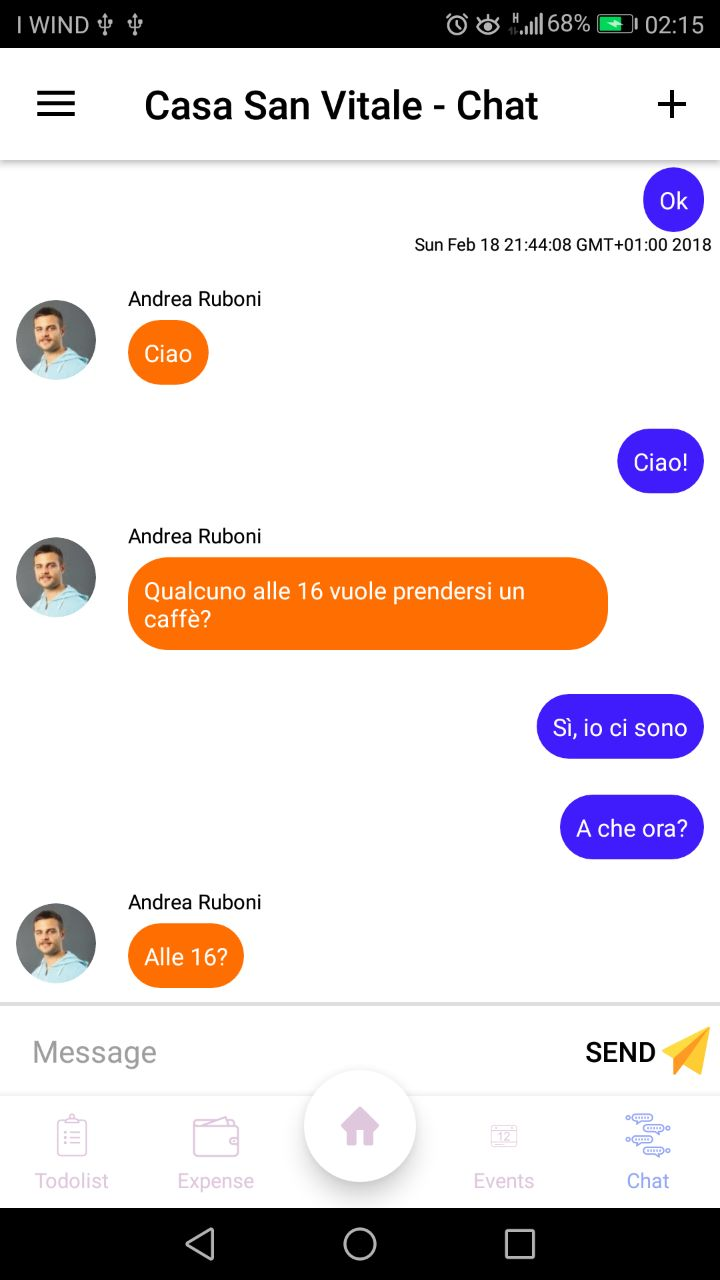
\includegraphics[width=0.3\textwidth]{immagini/app_chat.jpg}
  \caption{Schermata applicazione Chat}\label{fig:Schermata applicazione Chat}
\end{figure}

La chat come le precedenti pagine, utilizza il pattern MVP, di conseguenza all'interno del fragment verranno instanziati: il Presenter l'Adapter e implementata la View.\\
La chat per facilitare la visione dei messaggi ricevuti e inviati all'interno dell'Adapter prevede due differenti ViewHolder che differenziano il messaggio inviato da quello ricevuto.\\
La realizzazione di questa distinzione grafica fra i due tipi di messaggio richiede la creazione di una classe astratta ChatHolder che avesse come unico metodo la funzione ``bind'' e prendesse come parametro il messaggio, in modo tale che i due holder verranno implementati basandosi e estendendo questa classe.\\
Successivamente sono state sovrascritti i metodi ``getItemViewType'' e ``onCreateViewHolder'' del Fragment in modo tale da introdurre il controllo necessario per distinguere i messaggi.\\
All'interno del metodo getItemViewType, viene controllato il campo ``SenderUID'' del messaggio, corrispondente all'ID dell'utente che ha inviato il messaggio nel gruppo, questo ID viene poi confrontato con l'ID dell'utente loggato all'interno dell'applicazione in modo da restituire l'identificativo del layout da utilizzare nel ViewHolder.
\newpage
\begin{lstlisting}[language=kotlin,caption={Logica della funzione getItemViewType della Chat}]
when (senderUid == userUid) {
    false -> return R.layout.item_message_recived
    true -> return R.layout.item_message_sent
}
\end{lstlisting}
Una volta differenziato il tipo attraverso il metodo getItemViewType, è stata sovrascritto il metodo onCreateViewHolder che dovendo restituire un singolo Holder, come valore di ritorno restituisce un tipo ChatHolder (classe astratta implementata dalle due ViewHolder). In questo modo in base al tipo restituito da getItemViewType la classe onCreateViewHolder restituirà l'holder corrispondente al messaggio.
\begin{lstlisting}[language=kotlin,caption={Logica della funzione onCreateViewHolder della chat}]

when (viewType) {
           R.layout.item_message_sent -> holder = MessageChatSentHolder(itemView = view, dateOfLastMessage = lastItem?.timestamp)
           R.layout.item_message_recived -> holder = MessageChatRecivedHolder(itemView = view, dateOfLastMessage = lastItem?.timestamp)
       }
   \end{lstlisting}

\section{Supporto}
Il progetto è stato realizzato utilizzando librerie open source importante e gestite da Gradle, un programma per l'automazione dello sviluppo.\\
Gradle è stato progettato per automatizzare il processo di generazione di un progetto, facilitando l'aggiunta di librerie esterne, la compilazione finale del progetto comprese le sue dipendenze e l'aggiunta di test automatizzati.\\
La lista delle librerie utilizzate nel progetto possono essere divise in quattro categorie:
\begin{itemize}
    \item Librerie di supporto per Android e Kotlin
    \item Librerie SDK di Firebase
    \item Libreria per il supporto della programmazione reattiva
    \item Librerie per la gestione delle immagini
    \item Librerie per componenti grafici aggiuntivi
\end{itemize}

\newpage
\subsection{Librerie}
Le librerie offerte da Android per il supporto di funzionalità e componenti grafici aggiuntivi sono le seguenti:
\begin{table}[!h]
\begin{center}
\begin{tabular}{|l|p{6cm}|}
    \hline
\textbf{Libreria} & \textbf{Descrizione}\\ \hline
com.android.support:support & Libreria di supporto per Android  \\ \hline
com.android.support:appcompat & Supporto per i componenti grafici aggiuntivi \\ \hline
com.android.support:recyclerview & Widget personalizzabile simile al ListView ma più avanzato e flessibile \\ \hline
com.android.support:cardview & Componente per realizzare interfacce Material Design \\ \hline
com.android.support:design & Libreria di supporto per l'interfaccia Android  \\ \hline
com.android.support:constraint-layout & Layout personalizzabile \\ \hline
com.google.android:flexbox  & Layout personalizzabile Flex per Android  \\ \hline
com.android.support:customtabs & Libreria di supporto per il widget Tab  \\ \hline
android.arch.lifecycle:extensions & Supporto per Android Components Architecture \\ \hline
com.android.support:vector-drawable & Supporto per immagini svg e vettoriali  \\ \hline
android.arch.lifecycle:common-java8 &  Supporto per la gestone del lifecycle Android \\ \hline
org.jetbrains.kotlin:kotlin-stdlib-jre7 & Supporto per il linguaggio Kotlin su Android \\ \hline
\end{tabular}
\caption[Librerie Google del progetto]{Librerie Google del progetto}\label{tab:Librerie Google del progetto}
\end{center}
\end{table}

\newpage

Le librerie di supporto offerte da Firebase per utilizzare i suoi servizi sono le seguenti:

\begin{table}[!h]
\begin{center}
\begin{tabular}{|p{6cm}|p{7cm}|}
    \hline
\textbf{Libreria} & \textbf{Descrizione}\\ \hline
com.google.android.gms:play-services-auth  & Libreria di supporto per i servizi Google  \\ \hline
com.google.firebase:firebase-auth & SDK del servizio di autenticazione di Firebase \\ \hline
com.google.firebase:firebase-firestore & SDK per interfacciarsi con il database Firestore \\ \hline
com.google.firebase:firebase-storage & SDK per usufruire dello storage di Firebase  \\ \hline
com.google.firebase:firebase-messaging & SDK del servizio di messaggistica \\ \hline
com.firebase:firebase-jobdispatcher  & Supporto per lo scheduling e l'esecuzione in background\\ \hline
com.firebaseui:firebase-ui-auth & Libreria di supporto per il servizio Firebase-Auth  \\ \hline
com.firebaseui:firebase-ui-firestore & Libreria di supporto per il servizio Firestore  \\ \hline
com.firebaseui:firebase-ui-storage & Libreria di supporto per il servizio Storage  \\ \hline
com.facebook.android:facebook-android-sdk & SDK per l'accesso tramite il social Facebook \\ \hline
com.twitter.sdk.android:twitter-core & SDK per l'accesso tramite il social Twitter \\ \hline
\end{tabular}
\caption[Librerie Firebase del progetto]{Librerie Firebase del progetto}\label{tab:Librerie Firebase del progetto}
\end{center}
\end{table}

\newpage



Le librerie che offrono componenti grafici aggiuntivi sono le seguenti:

\begin{table}[!h]
\begin{center}
\begin{tabular}{|p{6cm}|p{7cm}|}
    \hline
\textbf{Libreria} & \textbf{Descrizione}\\ \hline
com.github.ittianyu: BottomNavigationViewEx  & Widget per il menu di navigazione  \\ \hline
com.stephentuso:welcome  & Libreria per mostrare pagine di presentazione e introduzione iniziali \\ \hline
com.shuhart.moneyedittext: moneyedittext-kotlin  & Widget per indicare l'ammontare di una spesa \\ \hline
br.com.simplepass:loading-button-android  & Widget che trasforma un Button in unna barra di caricamento  \\ \hline
com.github.Mariovc:ImagePicker  & Libreria di supporto per selezionare un'immagine dalla galleria del dispositivo  \\ \hline
com.github.bumptech.glide:glide & Libreria per la gestione delle immagini con funzionalità di caching \\ \hline
de.hdodenhof:circleimageview  & Libreria per visualizzare immagini con un bordo circolare \\ \hline
com.appeaser.sublimepickerlibrary: sublimepickerlibrary & Libreria per la selezione di una data dal calendario personalizzabile  \\ \hline
\end{tabular}
\caption[Librerie Firebase del progetto]{Librerie Firebase del progetto}\label{tab:Librerie Firebase del progetto}
\end{center}
\end{table}

\newpage
Infine le librerie di supporto per implementare la programmazione reattiva sono i seguenti:


\begin{table}[!h]
\begin{center}
\begin{tabular}{|l|p{8cm}|}
    \hline
\textbf{Libreria} & \textbf{Descrizione}\\ \hline
io.reactivex.rxjava2:rxjava:& Supporto dei costrutti della programmazione reattiva su Java  \\ \hline
io.reactivex.rxjava2:rxkotlin & Supporto per la programmazione reattiva su Kotlin  \\ \hline
io.reactivex.rxjava2:rxandroid & Supporto della libreria RxJava2 su Android  \\ \hline
\end{tabular}
\caption[Librerie di supporto per il Reactive programming]{Librerie di supporto per il Reactive programming}\label{tab:Librerie di supporto per il Reactive programming}
\end{center}
\end{table}

 \chapter{Sviluppo Server}                %crea il capitolo
%%%%%%%%%%%%%%%%%%%%%%%%%%%%%%%%%%%%%%%%%imposta l'intestazione di pagina
\lhead[\fancyplain{}{\bfseries\thepage}]{\fancyplain{}{\bfseries\rightmark}}
La realizzazione e lo sviluppo della parte server è stato facilitato dal servizio Firebase, che facilitava la creazione del database, la scrittura di regole di sicurezza e l'implementazione di script per il servizio Cloud Functions, la manutenzione dei server invece è stata interamente gestita da Firebase.

\section{Notifiche}
Gli utente appartenenti ad un gruppo riceveranno delle notifiche in tempo reale ogni volta che verrà aggiunto un nuovo contenuto all'interno dell'applicaziond, in particolare quando un utente aggiunge o completata una mansione, un evento o una spesa, oppure viene ricevuto un messaggio dalla chat.\\
Il servizio che consente di inviare messaggi ai dispositivi è Firebase Cloud Messaging e opera tipicamente attraverso le porte 5228 fino alle 5230, le richieste che vengono effettuate dall'applicazione al server FCM sono:
\begin{itemize}
    \item Creazione di un nuovo token attraverso l'SDK.
    \item Creazione di un gruppo comprendente più token.
    \item Aggiunta di un token all'interno di un gruppo di token.
\end{itemize}

La richiesta e il processo di generazione di un nuovo token per un nuovo client è automatizzata dall'SDK di FCM.
La creazione di un nuovo gruppo di utenti invece è effettuabile attraverso una richiesta HTTP POST ad un API, che restituisce un token, utilizzato come identificativo del gruppo.

\begin{lstlisting}[language=java,caption={Creazione di un token per il servizio FCM}]
https://android.googleapis.com/gcm/notification
Content-Type:application/json
Authorization:key=API_KEY
project_id:SENDER_ID
{
   "operation": "create",
   "notification_key_name": "appTesi",
   "registration_ids": ["4", "8", "15", "16", "23", "42"]
}
\end{lstlisting}

Una volta creato il gruppo è possibile aggiungere altri membri al gruppo, effettuando una richiesta simile alla precedente indicando come tipo di operazione "add" anzichè "create", che indica l'aggiunta di un nuovo token, oltre ad indicare il tipo di operazione la richiesta necessita del token del dispositivo da aggiungere al gruppo.

\begin{lstlisting}[language=java,caption={Creazione token FCM}]
https://android.googleapis.com/gcm/notification
Content-Type:application/json
Authorization:key=API_KEY
project_id:SENDER_ID

{
   "operation": "add",
   "notification_key_name": "appTesi",
   "registration_ids": ["7"]
}
\end{lstlisting}

\section{Cloud Functions}
I cambiamenti all'interno del database Firestore vengono monitorati utilizzando il servizio Cloud Functions che consentiva di scrivere script NodeJS eseguiti in base ai cambiamenti avvenuti nel database.\\
Gli script vengono salvati all'interno di un unico file, con l'estensione ".js", questo file conterrà tutte le funzioni che il Cloud Functions dovrà monitorare ed eseguire.\\
Il file principale utilizza due librerie per funzionare: ``Firebase-functions'' e ``firebase-admin'', che offrono le funzionalità utilizzabili dalle funzioni per interagire con Cloud Functions e con gli altri servizi Firebase.

\begin{lstlisting}[language=java,caption={Librerie utilizzate per interagire con il servizio Cloud Functions }]
// Definisco le librerie
let functions = require('firebase-functions');
let admin = require('firebase-admin');

//Inizializzo la libreria admin
admin.initializeApp(functions.config().firebase);
//Definisco ``firestore'' utilizzando il relativo modulo della libreria admin
const firestore = admin.firestore();
\end{lstlisting}

Ogni singola funzione invece è contrassegnata da un nome, il documento o la collezione del database da monitorare e l'evento ad esso associato.\\
Le funzioni scritte sono molto simili fra loro poichè monitorano solamente l'aggiunta di un nuovo elemento all'interno di una collezione o il cambiamento di un valore all'interno di un documento.\\

Prendendo in considerazione una funzione è possibile vedere quindi tutti gli elementi e le caratteristiche utilizzate per scrivere le funzioni, un esempio utilizzato per lo sviluppo della gestione della todolist è il seguente:\\
\newpage

\begin{lstlisting}[language=java,caption={Funzone Cloud Functions}]
exports.onGroupTodoCompleted = functions.firestore.document("groups/{groupsID}/todolist/{todoID}") .onUpdate(event => {
    const promises = [];
    const todo = event.data.data();
    const groupUIid = event.params.groupsID
    const getGroupTokenFCMPromise = firestore.collection("groups").doc(groupUIid).get()
    const prev_status = event.data.previous.data().status
    if (todo.status !== prev_status) {
        ...
    } else {
        return Promise.all(promises);
    }
});
\end{lstlisting}

In questa porzione di codice è possibile notare la struttura base di una funzione comprendente il nome (onGroupTodoCompleted), il riferimento alla collezione da monitorare (groups/{groupsID}/todolist/{todoID}) e l'evento (onUpdate).\\
Quando un documento all'interno della collezione ``todolist'' subisce una modifica viene confrontato il valore ``status'' della mansione precedente alla modifica, se questo valore è cambiato allora verrà inviata una notifica ai membri del gruppo altrimenti la funzione terminerà restituendo un Array vuoto.\\
Cloud Functions come citato in precedenza, permette di interagire anche con altri servizi Firebase, in questo caso il servizio con cui interagisce è Cloud Messaging, permettendo quindi di inviare una notifica ad uno o più dispositivi.\\
Un esempio di inivio di una notifica attraverso le Cloud Functions è il seguente:
\newpage

\begin{lstlisting}[language=java,caption={Funzone Cloud Functions}]
const groupTokenFCM = groupResponse.data().tokenFCM
var todotype = (todo.status === 'true') ? COMPLETED_TODO_TYPE : NEW_TODO_TYPE;
var payload = {
    "data": {
        "type": todotype, "name": todo.name, "sender": todo.created_by,
    }
};
const pushNotificationPromise = admin.messaging().sendToDeviceGroup(groupTokenFCM, payload)
return Promise.resolve(pushNotificationPromise){
    .then(function(response) {
        return Promise.all(promises);
    })
    .catch(function(error) {
        console.log("Error sending todo message:", error);
    })
}).catch(function(error) {
    console.log("Error sending todo message:", error);
})
\end{lstlisting}


\section{Sicurezza}
La sicurezza dei dati presenti sul database è fornita attraverso le Firestore Rules, un servizio integrato all'interno del database che permette di definire regole di accesso e validazione dei dati, attraverso una sintassi propria simile al Javascript.\\
I dati possono essere visualizzati solamente dagli utenti registrati, di conseguenza è stata creata una funzione ausiliare che verrà richiamata all'interno delle relative regole riguardanti le collezioni che utilizzano il controllo dell'accesso.


\begin{lstlisting}[language=java,caption={Firestore Rules Controllo autenticazione}]
function isUserAuthenticated() {
  return request.auth.uid != null;
}
\end{lstlisting}

Successivamente sono state definite le funzioni per controllare che l'utente faccia parte della mansione spesa o evento interno al gruppo.

\begin{lstlisting}[language=java,caption={Firestore Rules Controllo Visibilità}]
function userBelongsToGroup(userId) {
  return resource.data.users[userId] != null;
}
\end{lstlisting}
Queste funzioni vengono richiamate dalle regole da applicare alle collezioni, una particolarità utile è la possibilità di definire regole all'interno di sub-collezioni che sovascrivono parzialmente o totalmente le regole definite nella collezione esterna.
Un esempio è il seguente:

\begin{lstlisting}[language=java,caption={Firestore Rules Controllo Visibilità}]
match /groups/{groupsId} {
    allow read: if isUserAuthenticated();
    allow write, update, delete: if isUserAuthenticated() && userBelongsToGroup()

    match /todolist/{todolistId} {
      		allow write, update, delete if canUserReadItem()
          ...
    }
  ..
}
\end{lstlisting}

 %%%%%%%%%%%%%%%%%%%%%%%%%%%%%%%%%%%%%%%%%per fare le conclusioni
\chapter*{Conclusioni}
%%%%%%%%%%%%%%%%%%%%%%%%%%%%%%%%%%%%%%%%%imposta l'intestazione di pagina
\rhead[\fancyplain{}{\bfseries
Conclusioni}]{\fancyplain{}{\bfseries\thepage}}
\lhead[\fancyplain{}{\bfseries\thepage}]{\fancyplain{}{\bfseries
Conclusioni}}
\addcontentsline{toc}{chapter}{Conclusioni}

Lo stato dell'arte al momento in cui si scrive \`e un'applicazione in grado di gestire eventi, commissioni da svolgere, spese condivise e chat, attraverso l'utilizzo di un database aggiornato e consultabile in tempo reale, e la possibilità di gestire e creare le notifiche non appena avviene un cambiamento su di esso.\\
L'applicazione pur garantendo l'uso quotidiano delle funzionalità può essere ulteriormente migliorata, aggiungendo funzionalità, rendendola più stabile e riscriverla anche per la piattaforma iOS. Alcune idee in fase di sviluppo che verrano implementante sono le seguenti:
\begin{itemize}
  \item Chat di messaggistica istantanea anche fra i singoli componenti del gruppo
  \item Migliore flessibilità e funzionalità nella gestione degli eventi
  \item Nuovi informazioni inseribili all'interno di una spesa o commissione
  \item Permettere all'untente di partecipare a più di un gruppo contemporaneamente
  \item Scrivere l'applicazione per iOS utilizzando il linguaggio Swift
\end{itemize}
Attualmente il codice dell'applicazione è presente su Gitlab\footnote{http://gitlab.com/}, in una repository privata, non appena l'applicazione sarà considerata stabile e con le funzionalità desiderate, verrà resa pubblica.\\
L'applicazione è stata scritta utilizzando il linguaggio di programmazione Kotlin, a differenza del linguaggio Java solitamente utilizzato nello sviluppo di applicazioni mobili Android.\\ L'utilizzo di Kotlin come linguaggio per lo sviluppo dell'applicazione mi ha permesso di documentarmi sui nuovi concetti introdotti dal linguaggio e porlo a confronto con Java.\\
I risultati ricavabili dal confronto effettuato, sono stati significativi soprattutto per quanto riguarda le linee di codice, infatti prendendo in considerazione una parte del progetto scritta in Kotlin e confrontato con la relativa parte del progetto precedentemente scritta in Java, alcuni file che in Java richiedevono 140 linee di codice in Kotlin la stessa logica venica implementata in circa 80 linee per quanto.

riguarda le prestazioni e la memoria utilizzata invece si hanno valori trascurabili.\\



\begin{figure}[!hb]
  \centering
  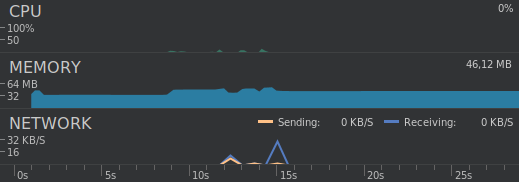
\includegraphics[width=0.8\textwidth]{immagini/app_java_memory_graph.png}
  \caption{Server Architettura}\label{fig:Android Studio }
\end{figure}

\begin{figure}[!hb]
  \centering
  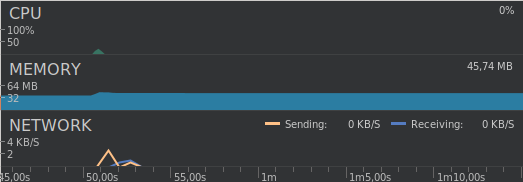
\includegraphics[width=0.8\textwidth]{immagini/app_kotlin_memory_graph.png}
  \caption{Server Architettura}\label{fig:Android Studio }
\end{figure}





\clearpage{\pagestyle{empty}\cleardoublepage}

 

\begin{thebibliography}{9}

\bibitem{latexcompanion}
Massimo Carli
\textit{Android 6. Guida per lo sviluppatore}.
Apogeo, 2016.

\bibitem{latexcompanion}
Stephen Samuel, Stefan Bocutiu
\textit{Programming Kotlin}.
Packtpub, 2017.

\bibitem{latexcompanion}
 Miloš Vasić
 \textit{Mastering Android Development with Kotlin}.
Packtpub, 2017.


\bibitem{latexcompanion}
Ronak K. Panchal,Akshay K. Patel \textit{A comparative study: Java Vs kotlin Programming in Android}.
International Journal of Innovative Trends in Engineering and Research, 2016.

\bibitem{ReactiveX}
ReactiveX documentation
\\\texttt{http://reactivex.io/documentation}

\bibitem{Android Developer }
Google Android Developer Documentation
\\\texttt{https://developer.android.com}

\bibitem{Firebase}
Google Firebase Documentation
\\\texttt{https://firebase.google.com/docs/}

\bibitem{Google I/O}
Google I/O - 2017
\\\texttt{https://events.google.com/io/}

\bibitem{Kotlin Lang}
Kotlin Language Documentation
\\\texttt{https://kotlinlang.org/docs/kotlin-docs.pdf}

\bibitem{Java Docs}
Oracle Java Documentation
\\\texttt{https://docs.oracle.com/}

\bibitem{Xamarin Guides}
Xamarin Android Google services guides
\\\texttt{https://developer.xamarin.com/guides/android/data-and-cloud-services/}

\bibitem{FirebaseUI-Android}
Libreria per la gestione dei servizi Firebase
\\\texttt{https://github.com/firebase/FirebaseUI-Android}

\bibitem{RxJava}
Libreria di supporto per la programmazione reattiva su Java
\\\texttt{https://github.com/ReactiveX/RxJava}

\bibitem{RxKotlin}
Libreria di supporto per la programmazione reattiva su Kotlin
\\\texttt{https://github.com/ReactiveX/RxAndroid}

\bibitem{RxAndroid}
Libreria di supporto per la programmazione reattiva su Android
\\\texttt{https://github.com/ReactiveX/RxKotlin}

\bibitem{BottomNavigationViewEx}
Libreria di supporto per il Widget del menu di navigazione
\\\texttt{https://github.com/ittianyu/BottomNavigationViewEx}

\bibitem{Welcome Android}
Libreria di supporto per mostrare pagine di presentazione e introduzione iniziali
\\\texttt{https://github.com/stephentuso/welcome-android}

\bibitem{MoneyEditText}
Libreria di supporto per il widget che consente di indicare l'ammontare di una spesa
\\\texttt{https://github.com/shuhart/MoneyEditText}

\bibitem{LoadingButtonAndroid }
Libreria di supporto per il widget che trasforma un Button in una barra di caricamento
\\\texttt{https://github.com/leandroBorgesFerreira/LoadingButtonAndroid}

\bibitem{Glide}
Libreria di supporto per la gestione delle immagini con funzionalità di caching
\\\texttt{https://github.com/bumptech/glide}

\bibitem{CircleImageView}
Libreria di supporto per visualizzare immagini con un bordo circolare
\\\texttt{https://github.com/hdodenhof/CircleImageView}

\bibitem{SublimePicker}
Libreria di supporto per la selezione di una data da un calendario personalizzabile
\\\texttt{https://github.com/vikramkakkar/SublimePicker/}

\bibitem{ImagePicker}
Libreria di supporto per selezionare un'immagine dalla galleria del dispositivo
\\\texttt{https://github.com/Mariovc/ImagePicker}

\bibitem{facebook Android SDK}
Libreria di supporto per l'accesso tramite il social network Facebook
\\\texttt{https://github.com/facebook/facebook-android-sdk}


\bibitem{Firebase Command Line Tools}
Tool a linea di comando per gestire i servizi Firebase
\\\texttt{https://github.com/facebook/facebook-android-sdk}


\bibitem{Firebase SDK for Cloud Functions}
Libreria di supporto per l'utilizzo del servizio Firebase Cloud Functions
\\\texttt{https://github.com/firebase/firebase-functions}




\end{thebibliography}

 

\chapter*{Ringraziamenti}
\thispagestyle{empty}
Un ringraziamento speciale alla mia famiglia che mi ha sempre sostenuto.


\end{document}
